%% ============================================================
%%  Assignment 1 – Image Filtering and Multiscale Processing
%%  Full Report  (Parts 1 · 2 · 3)
%%
%%  HOW TO COMPILE
%%  ──────────────
%%  1. Copy this file to the project root (next to outputs/ and images/).
%%  2. Run:   pdflatex report_full.tex
%%             pdflatex report_full.tex   (twice for ToC page numbers)
%%
%%  All \includegraphics paths are relative to the project root via
%%  the \graphicspath declarations below.
%% ============================================================
\documentclass[12pt,a4paper]{article}

% ---- Packages -----------------------------------------------
\usepackage[T1]{fontenc}
\usepackage[utf8]{inputenc}
\usepackage{lmodern}
\usepackage[margin=2.4cm, top=2.8cm, bottom=2.8cm]{geometry}
\usepackage{graphicx}
\usepackage{subcaption}
\usepackage{float}
\usepackage{booktabs}
\usepackage{array}
\usepackage{amsmath,amssymb}
\usepackage{xcolor}
\usepackage{listings}
\usepackage{hyperref}
\usepackage{microtype}
\usepackage{parskip}
\usepackage{titlesec}
\usepackage{fancyhdr}
\usepackage{caption}

% ---- Colour palette -----------------------------------------
\definecolor{accent}{RGB}{0,84,166}
\definecolor{codeblue}{RGB}{30,100,200}
\definecolor{codegray}{RGB}{120,120,120}
\definecolor{codegreen}{RGB}{0,128,60}
\definecolor{codered}{RGB}{180,30,30}

% ---- hyperref -----------------------------------------------
\hypersetup{
  colorlinks=true,
  linkcolor=accent,
  urlcolor=accent,
  citecolor=accent,
  pdftitle={Assignment 1 -- Image Filtering and Multiscale Processing},
  pdfauthor={Omar Khaled},
}

% ---- Section styling ----------------------------------------
\titleformat{\section}[block]
  {\large\bfseries\color{accent}}
  {\thesection}{1em}{}[\titlerule]
\titleformat{\subsection}[block]
  {\normalsize\bfseries\color{accent!80!black}}
  {\thesubsection}{1em}{}
\titleformat{\subsubsection}[block]
  {\normalsize\bfseries}
  {\thesubsubsection}{1em}{}

% ---- Code listings ------------------------------------------
\lstset{
  basicstyle=\ttfamily\small,
  keywordstyle=\color{codeblue}\bfseries,
  commentstyle=\color{codegreen}\itshape,
  stringstyle=\color{codered},
  numberstyle=\tiny\color{codegray},
  numbers=left,
  stepnumber=1,
  frame=single,
  breaklines=true,
  captionpos=b,
  language=Python,
  showstringspaces=false,
  tabsize=4,
  xleftmargin=1.5em,
}

% ---- Image path root ----------------------------------------
%  All paths are relative to the directory where pdflatex is run
%  (= the project root).
\graphicspath{
  {outputs/part2_1/apple-orange/}
  {outputs/part2_1/man-cat/}
  {outputs/part2_1/cat-tiger/}
  {outputs/part2_1/dodge-motorcycle/}
  {outputs/part2_1/favorite/}
  {outputs/part2_2/}
  {outputs/part2_3/}
  {outputs/part2_3/gaussian_pyramid/}
  {outputs/part2_3/laplacian_pyramid/}
  {outputs/part2_4/apple-orange/}
  {outputs/part2_4/eye-on-hand/}
  {outputs/part2_4/cat-on-sunflower/}
  {outputs/part2_4/face-on-apple/}
  {images/part2_frequencies/}
}

% ---- Caption style ------------------------------------------
\captionsetup{
  font=small,
  labelfont={bf,color=accent},
  labelsep=period,
  skip=4pt,
}

% ---- Header/Footer ------------------------------------------
\pagestyle{fancy}
\fancyhf{}
\fancyhead[L]{\small\color{accent}\textbf{Assignment 1 -- Image Filtering \& Multiscale Processing}}
\fancyhead[R]{\small\color{gray}Omar Khaled}
\fancyfoot[C]{\small\thepage}
\renewcommand{\headrulewidth}{0.4pt}

% ============================================================
\begin{document}
% ============================================================

%% ---- Title page -------------------------------------------
\begin{titlepage}
  \centering
  \vspace*{2cm}
  {\Huge\bfseries\color{accent} Assignment 1\par}
  \vspace{0.5em}
  {\Large\bfseries Image Filtering and Multiscale Processing\par}
  \vspace{2em}
  \rule{0.7\linewidth}{1pt}
  \vspace{1.5em}

  {\large\bfseries Omar Khaled\par}
  \vspace{0.5em}
  {\normalsize Computer Vision Course\par}
  \vspace{2em}
  {\normalsize\today\par}

  \vfill
  \begin{abstract}
    \noindent
    This report presents the implementation and results for all three parts of
    Assignment~1.
    \textbf{Part~1} implements 2D convolution from scratch (loop, vectorised,
    and separable), finite-difference edge detection, and derivative-of-Gaussian
    (DoG) edge detection.
    \textbf{Part~2} covers frequency-domain analysis through hybrid images
    (\S\ref{sec:21}), anti-aliasing with Gaussian pre-filtering (\S\ref{sec:22}),
    Gaussian and Laplacian pyramids (\S\ref{sec:23}), and multiresolution image
    blending (\S\ref{sec:24}).
    \textbf{Part~3} implements seam-carving for content-aware image resizing.
    All output images are included inline; each section opens with a brief
    description of the method, states all parameters, shows the key images,
    and provides a focused discussion of the results.
  \end{abstract}
\end{titlepage}

\tableofcontents
\newpage

%%=============================================================
\section{Part 1: Filters and Edges}
%%=============================================================

\subsection{Part 1.1 \texorpdfstring{---}{-} Convolution from Scratch}

All three implementations (\texttt{convolve\_loop}, \texttt{convolve\_vectorized},
\texttt{convolve\_separable}) return same-sized outputs with zero padding.
Benchmarks were recorded on a single $256\times256$ image with Gaussian kernels
of increasing size (one run per method and kernel size).

\begin{table}[H]
  \centering
  \caption{Convolution benchmark (single run, milliseconds).}
  \label{tab:conv_bench}
  \begin{tabular}{lrrr}
    \toprule
    \textbf{Kernel} & \textbf{Loop (ms)} & \textbf{Vectorised (ms)} & \textbf{Separable (ms)} \\
    \midrule
    $3\times3$   &    354.42 &   2.32 & 1.71 \\
    $5\times5$   &    976.75 &   3.31 & 1.72 \\
    $7\times7$   &  3483.22  &  21.09 & 6.36 \\
    $15\times15$ & 29288.91  &  65.54 & 6.88 \\
    $31\times31$ & 97831.67  &  55.06 & 3.72 \\
    \bottomrule
  \end{tabular}
\end{table}

The loop implementation's cost grows with \emph{kernel area} because every
multiply-add is a Python operation.  The vectorised implementation moves the
same work into NumPy, yielding a large speedup.  The separable implementation
exploits the rank-1 structure of a Gaussian kernel (factored into a column and
a row vector), so its cost grows with \emph{kernel width} rather than area,
making it especially efficient for large kernels.

Environment: Python 3.13.5, NumPy 2.3.1, SciPy 1.16.0.  Timings are from
one-run measurements; small fluctuations between sizes reflect cache and
system-load variation.

\subsection{Part 1.2 \texorpdfstring{---}{-} Finite Difference Edge Detection}

\textbf{Image:} \texttt{images/part1\_filters/facade.png}
(736$\times$670 px, grayscale, intensities in $[0,1]$).

\textbf{Threshold:} 0.20 marks 13.1\,\% of pixels as edges, giving a useful
balance of facade detail without overwhelming noise.  Threshold 0.15 marks
18.6\,\%, threshold 0.25 marks 9.4\%.

\textbf{Frame artefacts:} Zero-padding creates an artificial intensity jump at
the image border (comparing real pixels to zeros), producing edge lines along
the frame.  These are padding artefacts, not real object boundaries; they
disappear in Part~2 when reflection padding is used.

\subsection{Part 1.3 \texorpdfstring{---}{-} Derivative of Gaussian (DoG) Edge Detection}

\textbf{Image:} Same facade image.
\textbf{Parameters:} $\sigma=2.0$, threshold $=0.08$ (marks 11.7\,\% of pixels).

Blurring before differentiation suppresses small-scale intensity changes, so
the DoG edge map is substantially cleaner than the finite-difference map.
Smoothing spreads the boundary artefact over the DoG kernel's support.  The
Gaussian kernel is normalised only for display; processing uses the original
values.

%%=============================================================
\section{Part 2: Frequencies, Pyramids, and Blending}
%%=============================================================

%%-----------------------------------------------------------
\subsection{Part 2.1 \texorpdfstring{---}{-} Hybrid Images}
\label{sec:21}
%%-----------------------------------------------------------

\subsubsection{Method}

A \emph{hybrid image} is constructed by adding the low-pass version of one
image to the high-pass version of a second:

\begin{equation}
  H \;=\; \underbrace{G_{\sigma_{\ell}} * I_1}_{\text{low-pass}}
        + \underbrace{I_2 - G_{\sigma_{h}} * I_2}_{\text{high-pass}},
  \label{eq:hybrid}
\end{equation}

where $G_{\sigma}$ is a Gaussian of standard deviation $\sigma$ and
`$*$' denotes 2D convolution.  At close viewing distance the eye resolves
fine detail and perceives $I_2$; at a distance only coarse structure is
visible and the viewer perceives $I_1$.

Both Gaussians use \textbf{reflected padding} (\texttt{padding\_mode="reflect"}),
implemented in \texttt{hybrid\_images.py} via \texttt{convolve\_separable}.
The second image is aligned to the first by two corresponding point pairs
(e.g.\ left-eye and right-eye centres), determining a similarity
transformation (scale, rotation, translation).

All three pairs use $\sigma_{\ell}=4$, $\sigma_{h}=4$ (values chosen by
visual inspection of the hybrid).

\subsubsection{Pair 1 \texorpdfstring{---}{-} Man / Cat (Required Starter Pair)}

\textbf{Low-pass image:} Man portrait (\texttt{hybrid\_man.jpg}).
\textbf{High-pass image:} Cat (\texttt{hybrid\_cat.jpg}).
Alignment points: left eye $(299, 341)$\,/\,$(443, 332)$ in the man;
$(605, 290)$\,/\,$(760, 372)$ in the cat.

\begin{figure}[H]
  \centering
  \begin{subfigure}[b]{0.32\textwidth}
    \includegraphics[width=\textwidth]{first_image.png}
    \caption{Man (low-pass input).}
  \end{subfigure}\hfill
  \begin{subfigure}[b]{0.32\textwidth}
    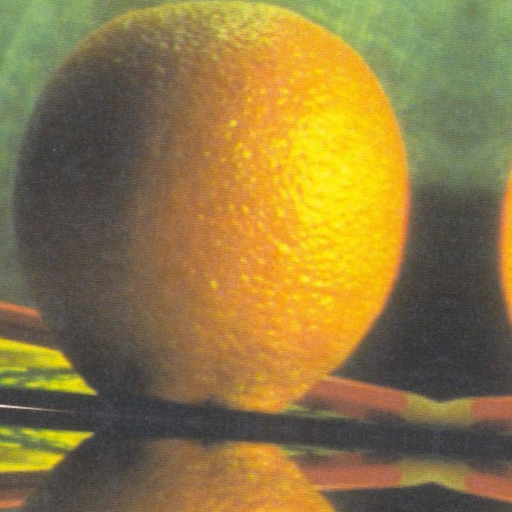
\includegraphics[width=\textwidth]{aligned_second_image.png}
    \caption{Cat (aligned, high-pass input).}
  \end{subfigure}\hfill
  \begin{subfigure}[b]{0.32\textwidth}
    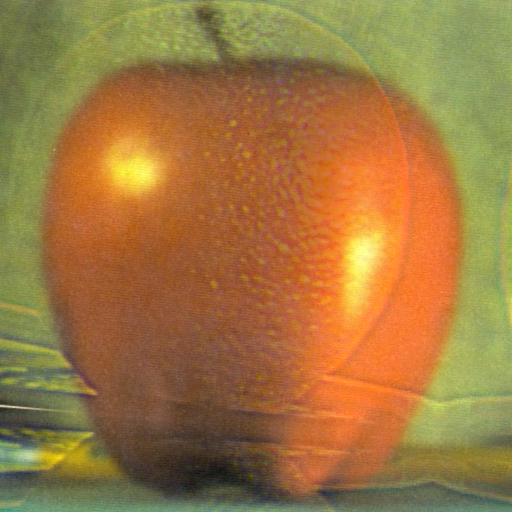
\includegraphics[width=\textwidth]{hybrid.png}
    \caption{Hybrid result.}
  \end{subfigure}

  \vspace{0.6em}

  \begin{subfigure}[b]{0.45\textwidth}
    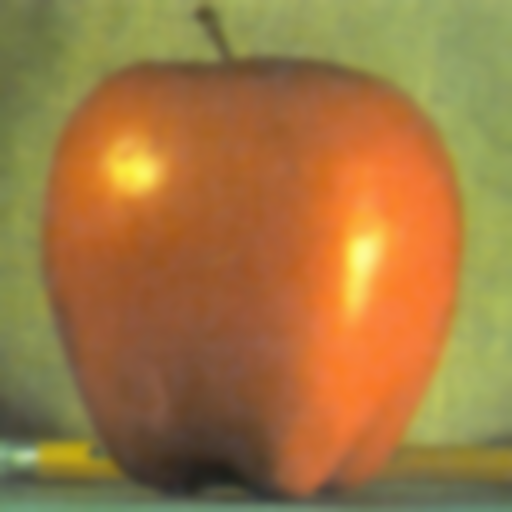
\includegraphics[width=\textwidth]{low_pass_first.png}
    \caption{Low-pass filtered man ($\sigma_{\ell}=4$).}
  \end{subfigure}\hfill
  \begin{subfigure}[b]{0.45\textwidth}
    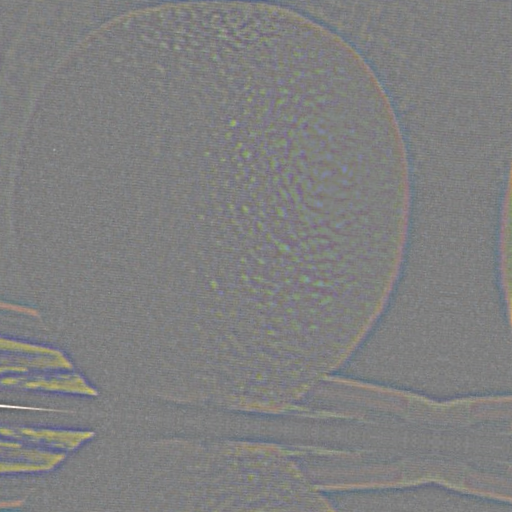
\includegraphics[width=\textwidth]{high_pass_second.png}
    \caption{High-pass filtered cat ($\sigma_{h}=4$).}
  \end{subfigure}
  \caption{\textbf{Man $\to$ Cat hybrid (pair~1).}
    Close up: cat's fur texture and whiskers dominate.
    At distance: the man's blurred portrait is perceived.}
  \label{fig:mancat}
\end{figure}

\subsubsection{Pair 2 \texorpdfstring{---}{-} Cat / Tiger}

\textbf{Low-pass:} Domestic cat (\texttt{cat.jpg}).
\textbf{High-pass:} Tiger (\texttt{Tiger.jpg}).
Alignment on matching eye centres.

\begin{figure}[H]
  \centering
  \begin{subfigure}[b]{0.32\textwidth}
    \includegraphics[width=\textwidth]{first_image.png}
    \caption{Cat (low-pass input).}
  \end{subfigure}\hfill
  \begin{subfigure}[b]{0.32\textwidth}
    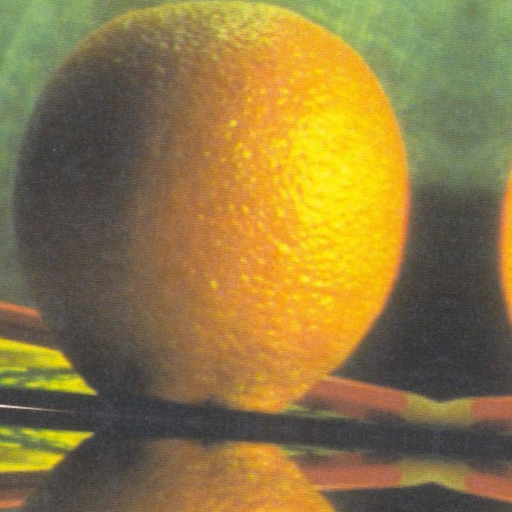
\includegraphics[width=\textwidth]{aligned_second_image.png}
    \caption{Tiger (aligned, high-pass input).}
  \end{subfigure}\hfill
  \begin{subfigure}[b]{0.32\textwidth}
    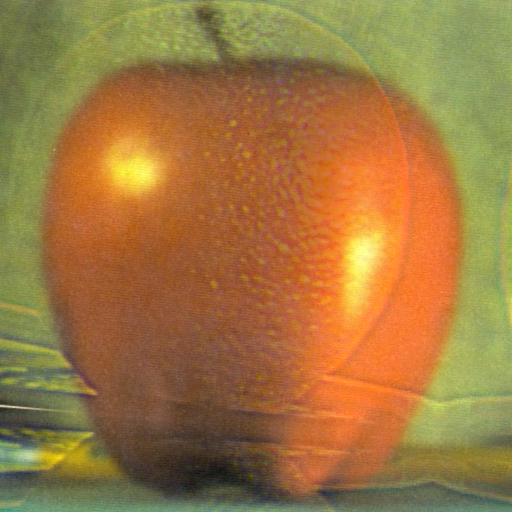
\includegraphics[width=\textwidth]{hybrid.png}
    \caption{Hybrid result.}
  \end{subfigure}

  \vspace{0.6em}

  \begin{subfigure}[b]{0.45\textwidth}
    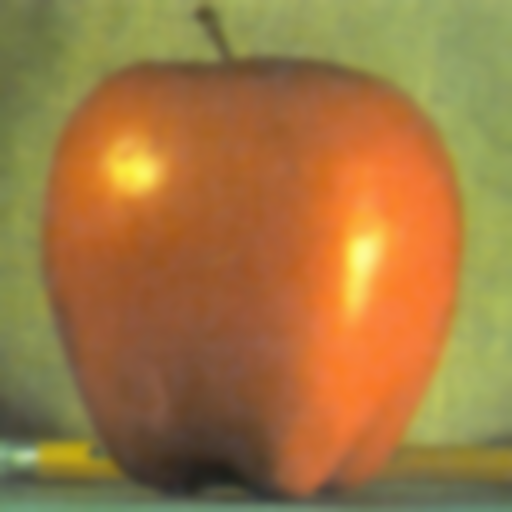
\includegraphics[width=\textwidth]{low_pass_first.png}
    \caption{Low-pass filtered cat.}
  \end{subfigure}\hfill
  \begin{subfigure}[b]{0.45\textwidth}
    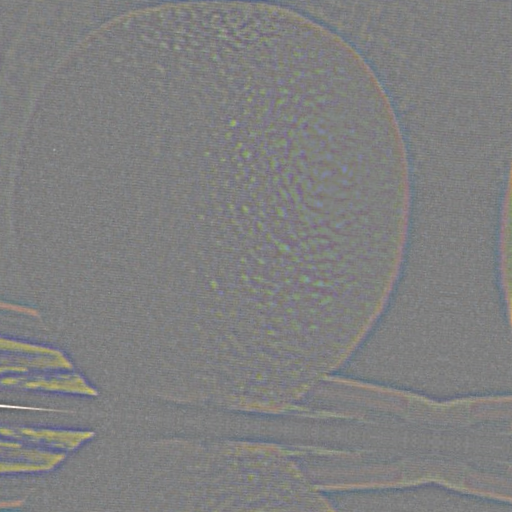
\includegraphics[width=\textwidth]{high_pass_second.png}
    \caption{High-pass filtered tiger.}
  \end{subfigure}
  \caption{\textbf{Cat $\to$ Tiger hybrid (pair~2).}
    The shared facial geometry (eye spacing, snout width, ear placement)
    makes the transition especially convincing.}
  \label{fig:cattiger}
\end{figure}

\subsubsection{Pair 3 \texorpdfstring{---}{-} Dodge Challenger / Kawasaki Motorcycle}

\textbf{Low-pass:} Dodge Challenger (front view).
\textbf{High-pass:} Kawasaki Ninja ZX-10RR (front view).
Alignment on front-wheel-centre and headlight correspondence.

\begin{figure}[H]
  \centering
  \begin{subfigure}[b]{0.32\textwidth}
    \includegraphics[width=\textwidth]{first_image.png}
    \caption{Dodge Challenger (low-pass input).}
  \end{subfigure}\hfill
  \begin{subfigure}[b]{0.32\textwidth}
    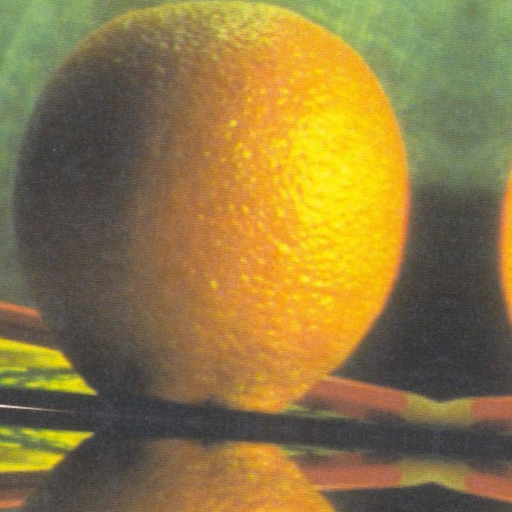
\includegraphics[width=\textwidth]{aligned_second_image.png}
    \caption{Kawasaki (aligned, high-pass input).}
  \end{subfigure}\hfill
  \begin{subfigure}[b]{0.32\textwidth}
    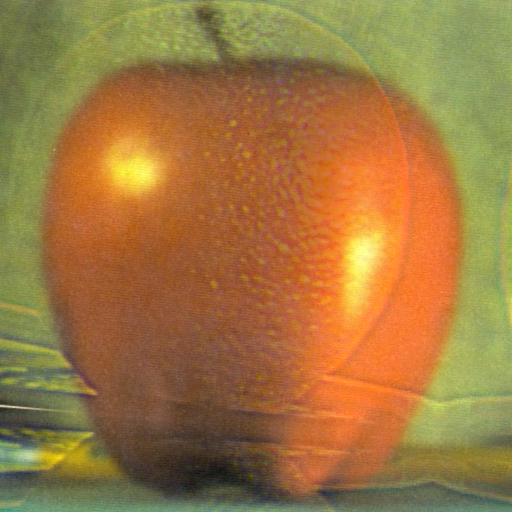
\includegraphics[width=\textwidth]{hybrid.png}
    \caption{Hybrid result.}
  \end{subfigure}

  \vspace{0.6em}

  \begin{subfigure}[b]{0.45\textwidth}
    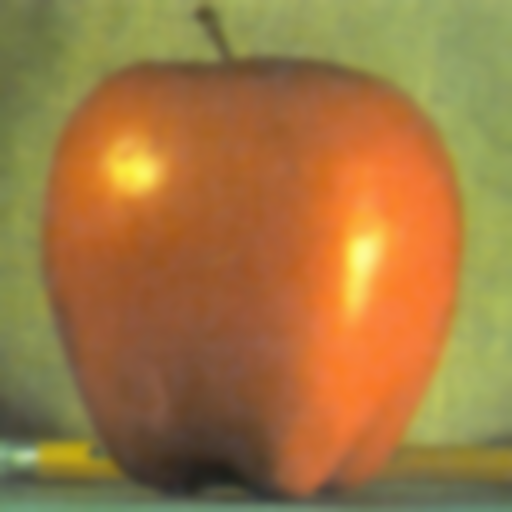
\includegraphics[width=\textwidth]{low_pass_first.png}
    \caption{Low-pass filtered Dodge.}
  \end{subfigure}\hfill
  \begin{subfigure}[b]{0.45\textwidth}
    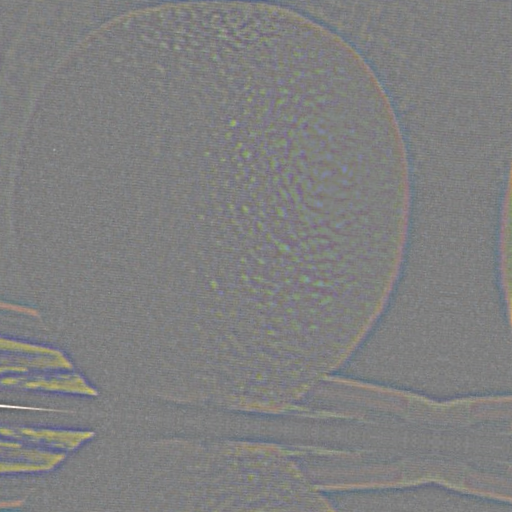
\includegraphics[width=\textwidth]{high_pass_second.png}
    \caption{High-pass filtered motorcycle.}
  \end{subfigure}
  \caption{\textbf{Dodge $\to$ Kawasaki hybrid (pair~3).}
    Close up: motorcycle spokes and fairing detail are visible.
    At distance: the wide-body muscle-car silhouette dominates.}
  \label{fig:vehicle}
\end{figure}

% ==================================================================
\subsubsection{Favourite Pair \texorpdfstring{---}{-} Man / Cat with Fourier Analysis}
\label{sec:21fav}
% ==================================================================

The man--cat pair is selected as the favourite because the facial geometry
aligns closely, producing a compelling multi-scale percept.
Figures~\ref{fig:fav_spatial} and~\ref{fig:fav_spectra} show all five
spatial stages and their centred log-magnitude Fourier spectra.

\begin{figure}[H]
  \centering
  \begin{subfigure}[b]{0.18\textwidth}
    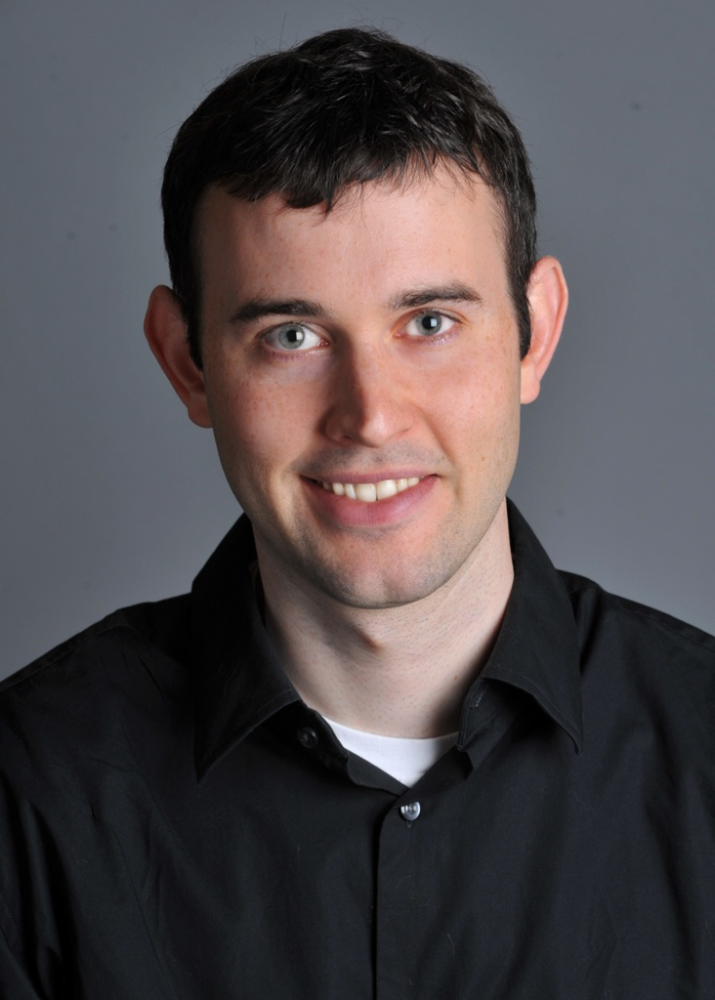
\includegraphics[width=\textwidth]{image_01_man.png}
    \caption{Man\\\footnotesize(original).}
  \end{subfigure}\hfill
  \begin{subfigure}[b]{0.18\textwidth}
    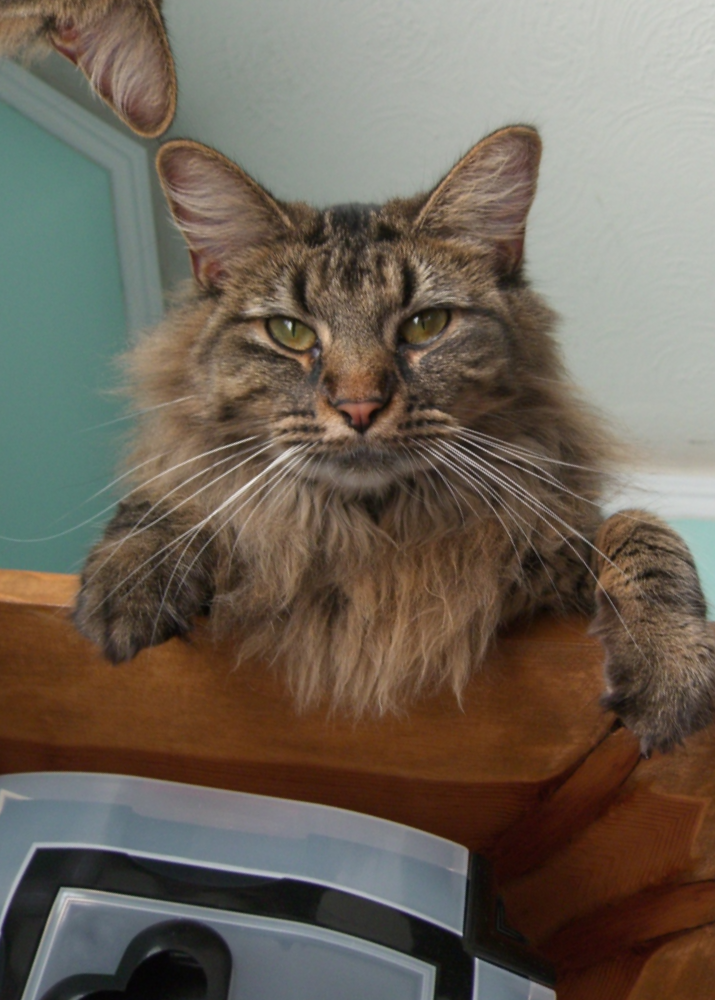
\includegraphics[width=\textwidth]{image_02_aligned_cat.png}
    \caption{Cat\\\footnotesize(aligned).}
  \end{subfigure}\hfill
  \begin{subfigure}[b]{0.18\textwidth}
    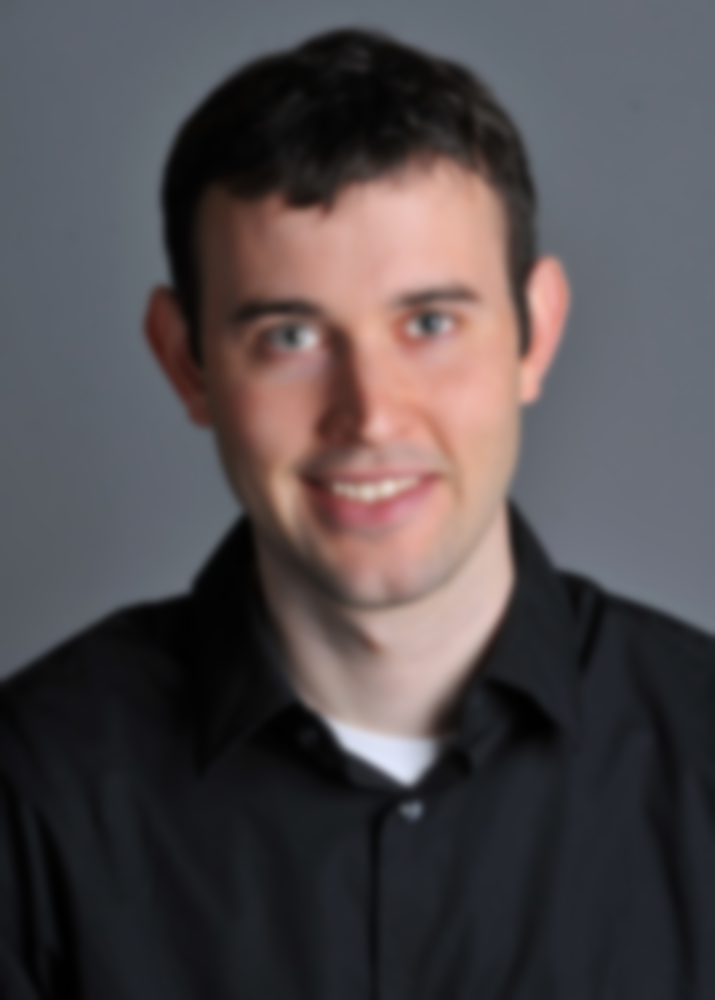
\includegraphics[width=\textwidth]{image_03_low_pass_man.png}
    \caption{Low-pass\\\footnotesize man.}
  \end{subfigure}\hfill
  \begin{subfigure}[b]{0.18\textwidth}
    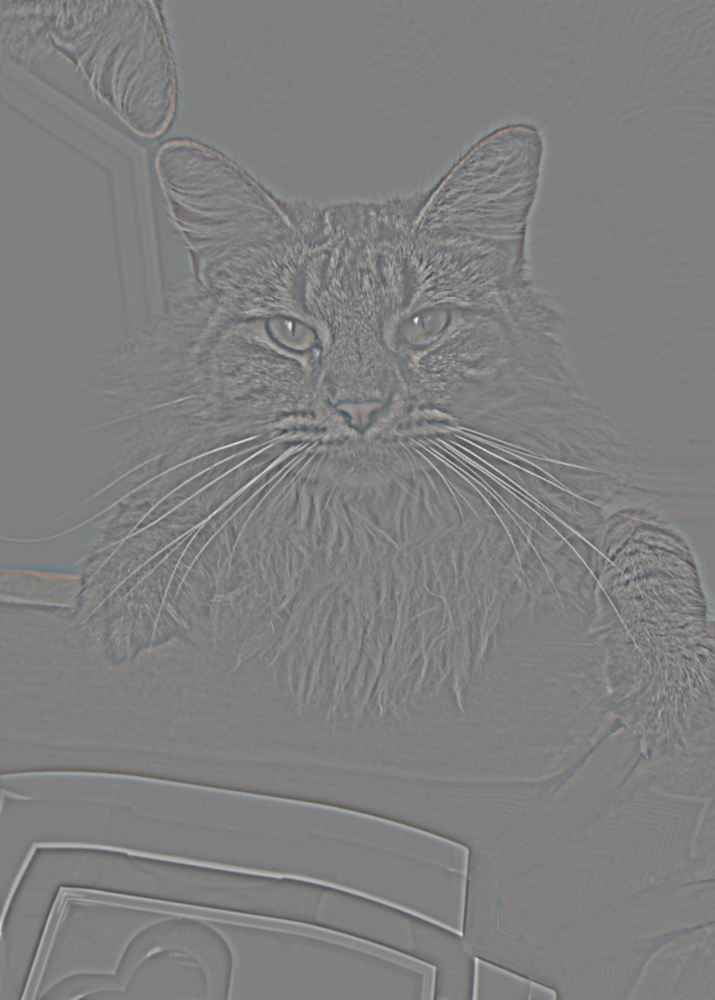
\includegraphics[width=\textwidth]{image_04_high_pass_cat.png}
    \caption{High-pass\\\footnotesize cat.}
  \end{subfigure}\hfill
  \begin{subfigure}[b]{0.18\textwidth}
    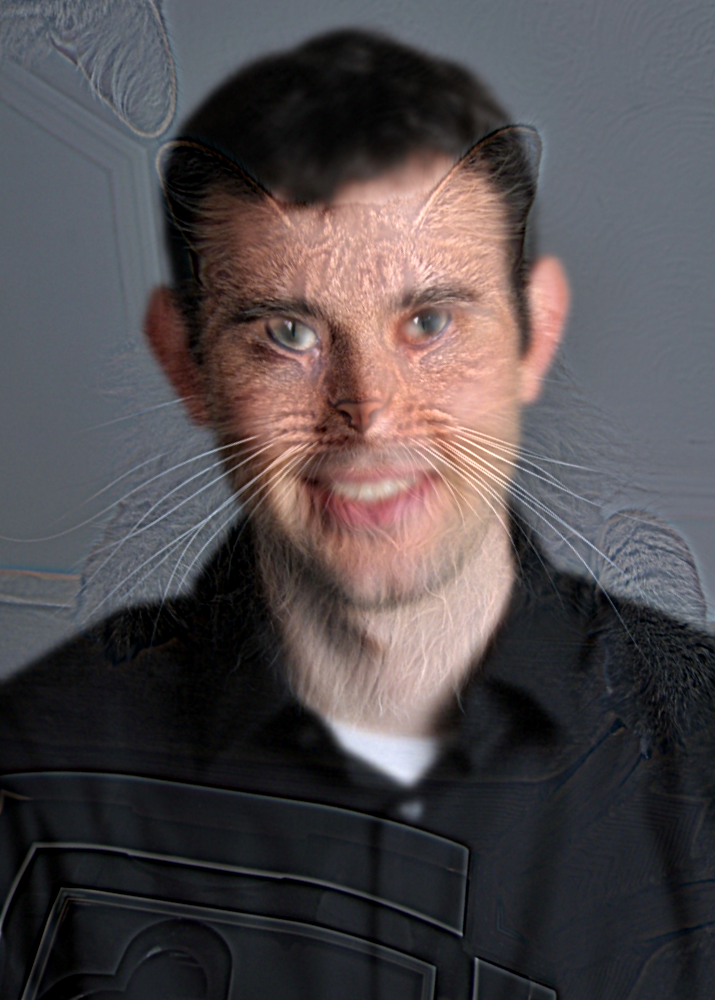
\includegraphics[width=\textwidth]{image_05_hybrid.png}
    \caption{Hybrid.}
  \end{subfigure}
  \caption{Favourite pair (man--cat) --- five spatial stages.}
  \label{fig:fav_spatial}
\end{figure}

\begin{figure}[H]
  \centering
  \begin{subfigure}[b]{0.18\textwidth}
    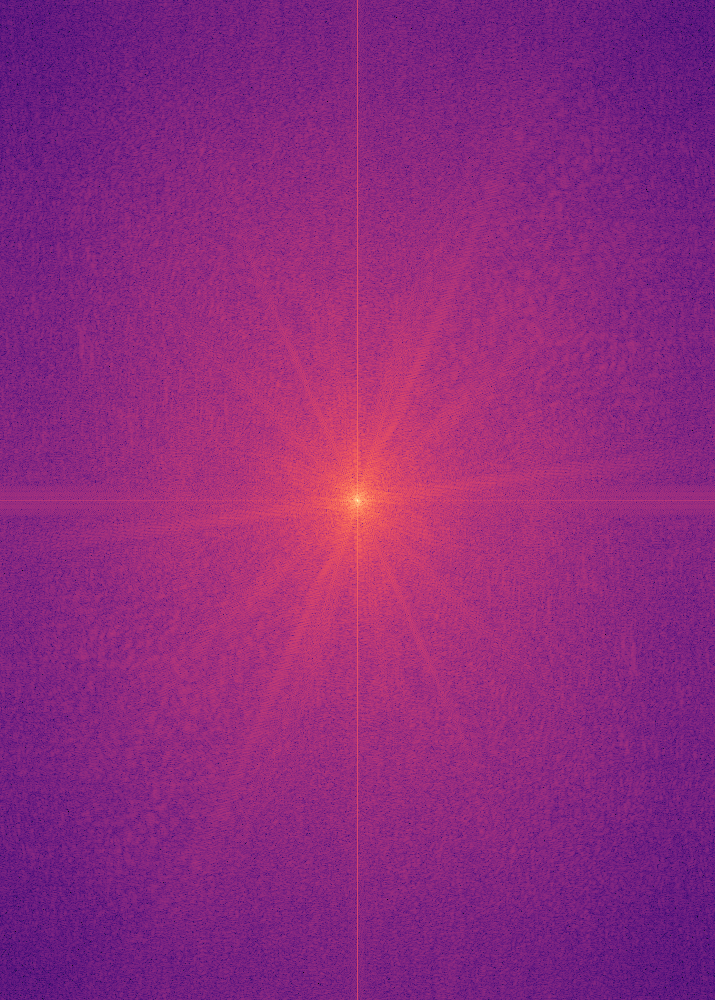
\includegraphics[width=\textwidth]{spectrum_01_man.png}
    \caption{Spectrum:\\\footnotesize man.}
  \end{subfigure}\hfill
  \begin{subfigure}[b]{0.18\textwidth}
    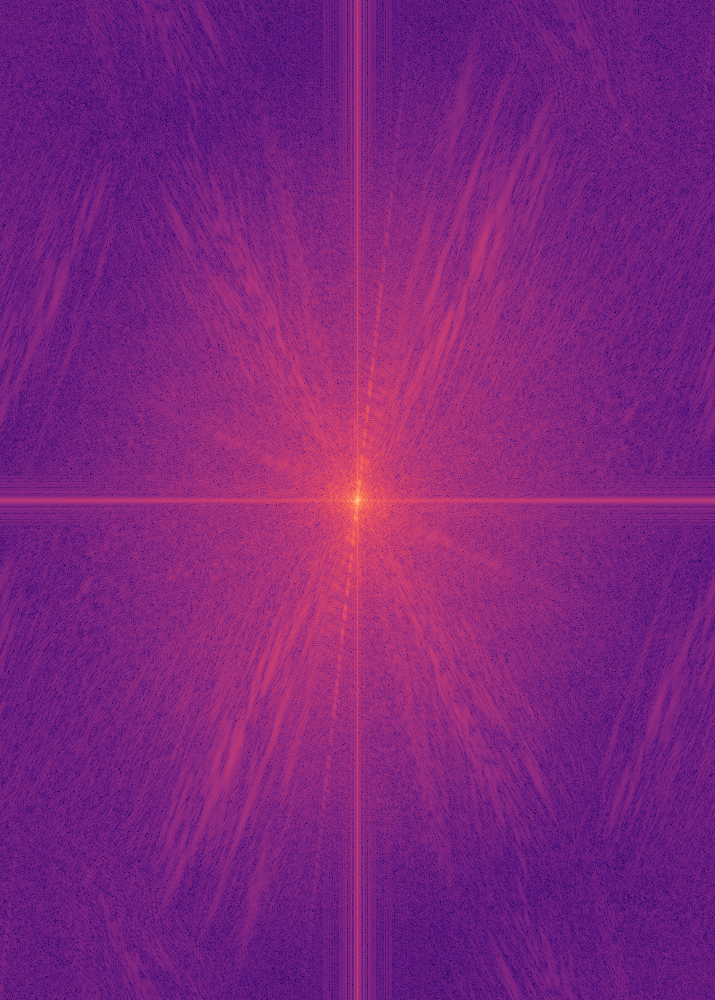
\includegraphics[width=\textwidth]{spectrum_02_aligned_cat.png}
    \caption{Spectrum:\\\footnotesize cat.}
  \end{subfigure}\hfill
  \begin{subfigure}[b]{0.18\textwidth}
    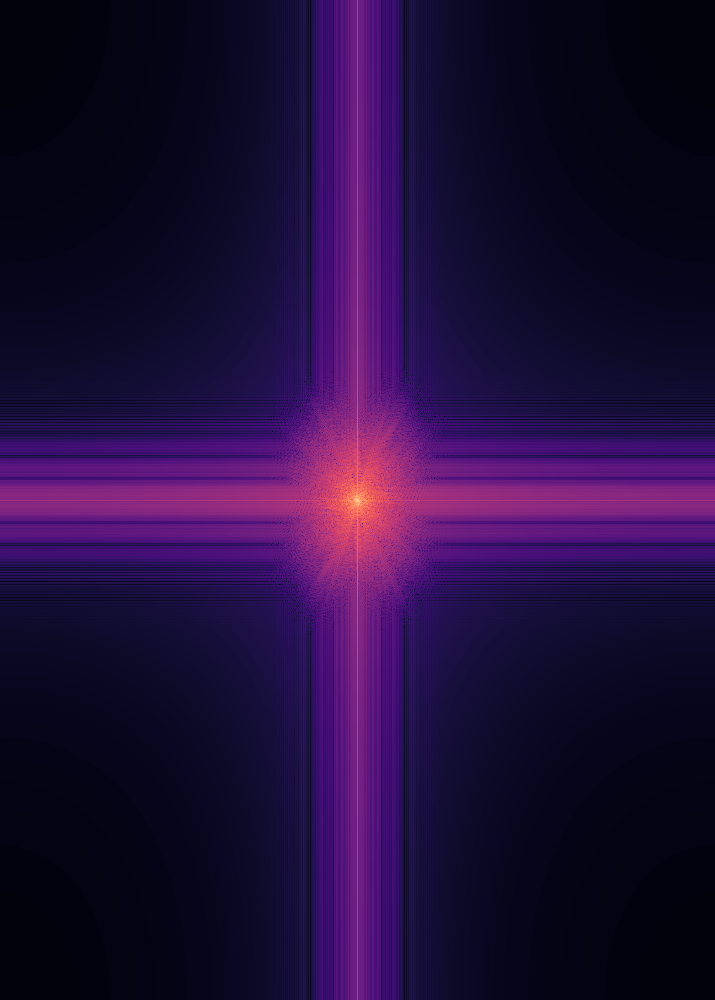
\includegraphics[width=\textwidth]{spectrum_03_low_pass_man.png}
    \caption{Spectrum:\\\footnotesize low-pass.}
  \end{subfigure}\hfill
  \begin{subfigure}[b]{0.18\textwidth}
    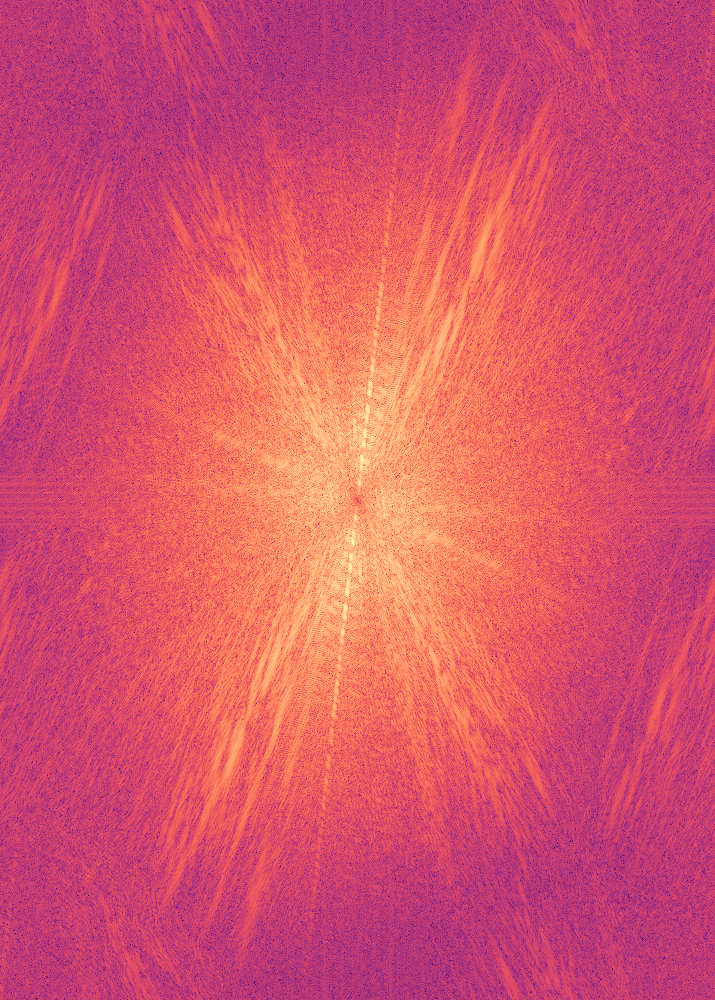
\includegraphics[width=\textwidth]{spectrum_04_high_pass_cat.png}
    \caption{Spectrum:\\\footnotesize high-pass.}
  \end{subfigure}\hfill
  \begin{subfigure}[b]{0.18\textwidth}
    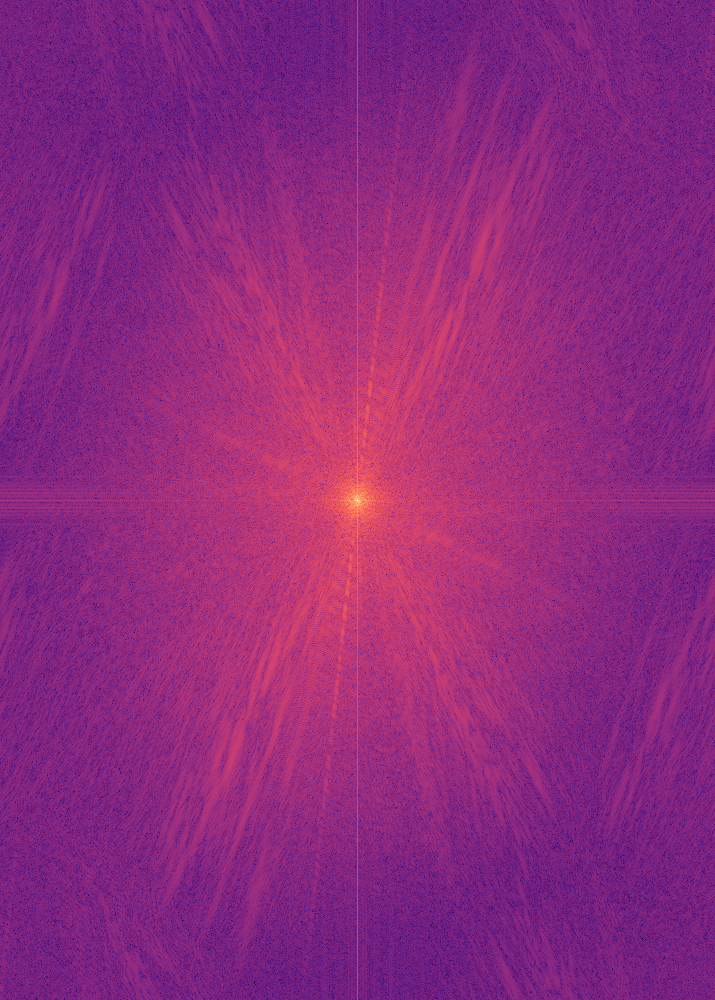
\includegraphics[width=\textwidth]{spectrum_05_hybrid.png}
    \caption{Spectrum:\\\footnotesize hybrid.}
  \end{subfigure}
  \caption{Favourite pair (man--cat) --- centred log-magnitude Fourier spectra.}
  \label{fig:fav_spectra}
\end{figure}

\paragraph{How to read the spectra.}
Each image shows $\log(1+|\hat{f}(u,v)|)$ centred at DC (zero frequency).
Bright regions indicate high energy at those spatial frequencies.

\begin{itemize}
  \item \textbf{Man (a,b):} Energy at all frequencies; the bright cross
    reflects the dominant horizontal and vertical structures of the face.
  \item \textbf{Low-pass man (c):} Only the central low-frequency disk survives;
    the Gaussian acts as a circular low-pass filter in the frequency domain,
    attenuating the outer ring.
  \item \textbf{Cat (b):} Similar full-band spectrum.
  \item \textbf{High-pass cat (d):} The central blob is suppressed (DC and
    low frequencies removed); the outer high-frequency ring dominates,
    creating an almost annular spectrum.
  \item \textbf{Hybrid (e):} \emph{Dual-band} spectrum: strong central disk
    from the man's low frequencies plus the outer ring from the cat's high
    frequencies.  This dual structure directly explains the perceptual switch:
    the visual system integrates low frequencies at distance (seeing the man)
    and resolves high frequencies close up (seeing the cat).
\end{itemize}

\begin{figure}[H]
  \centering
  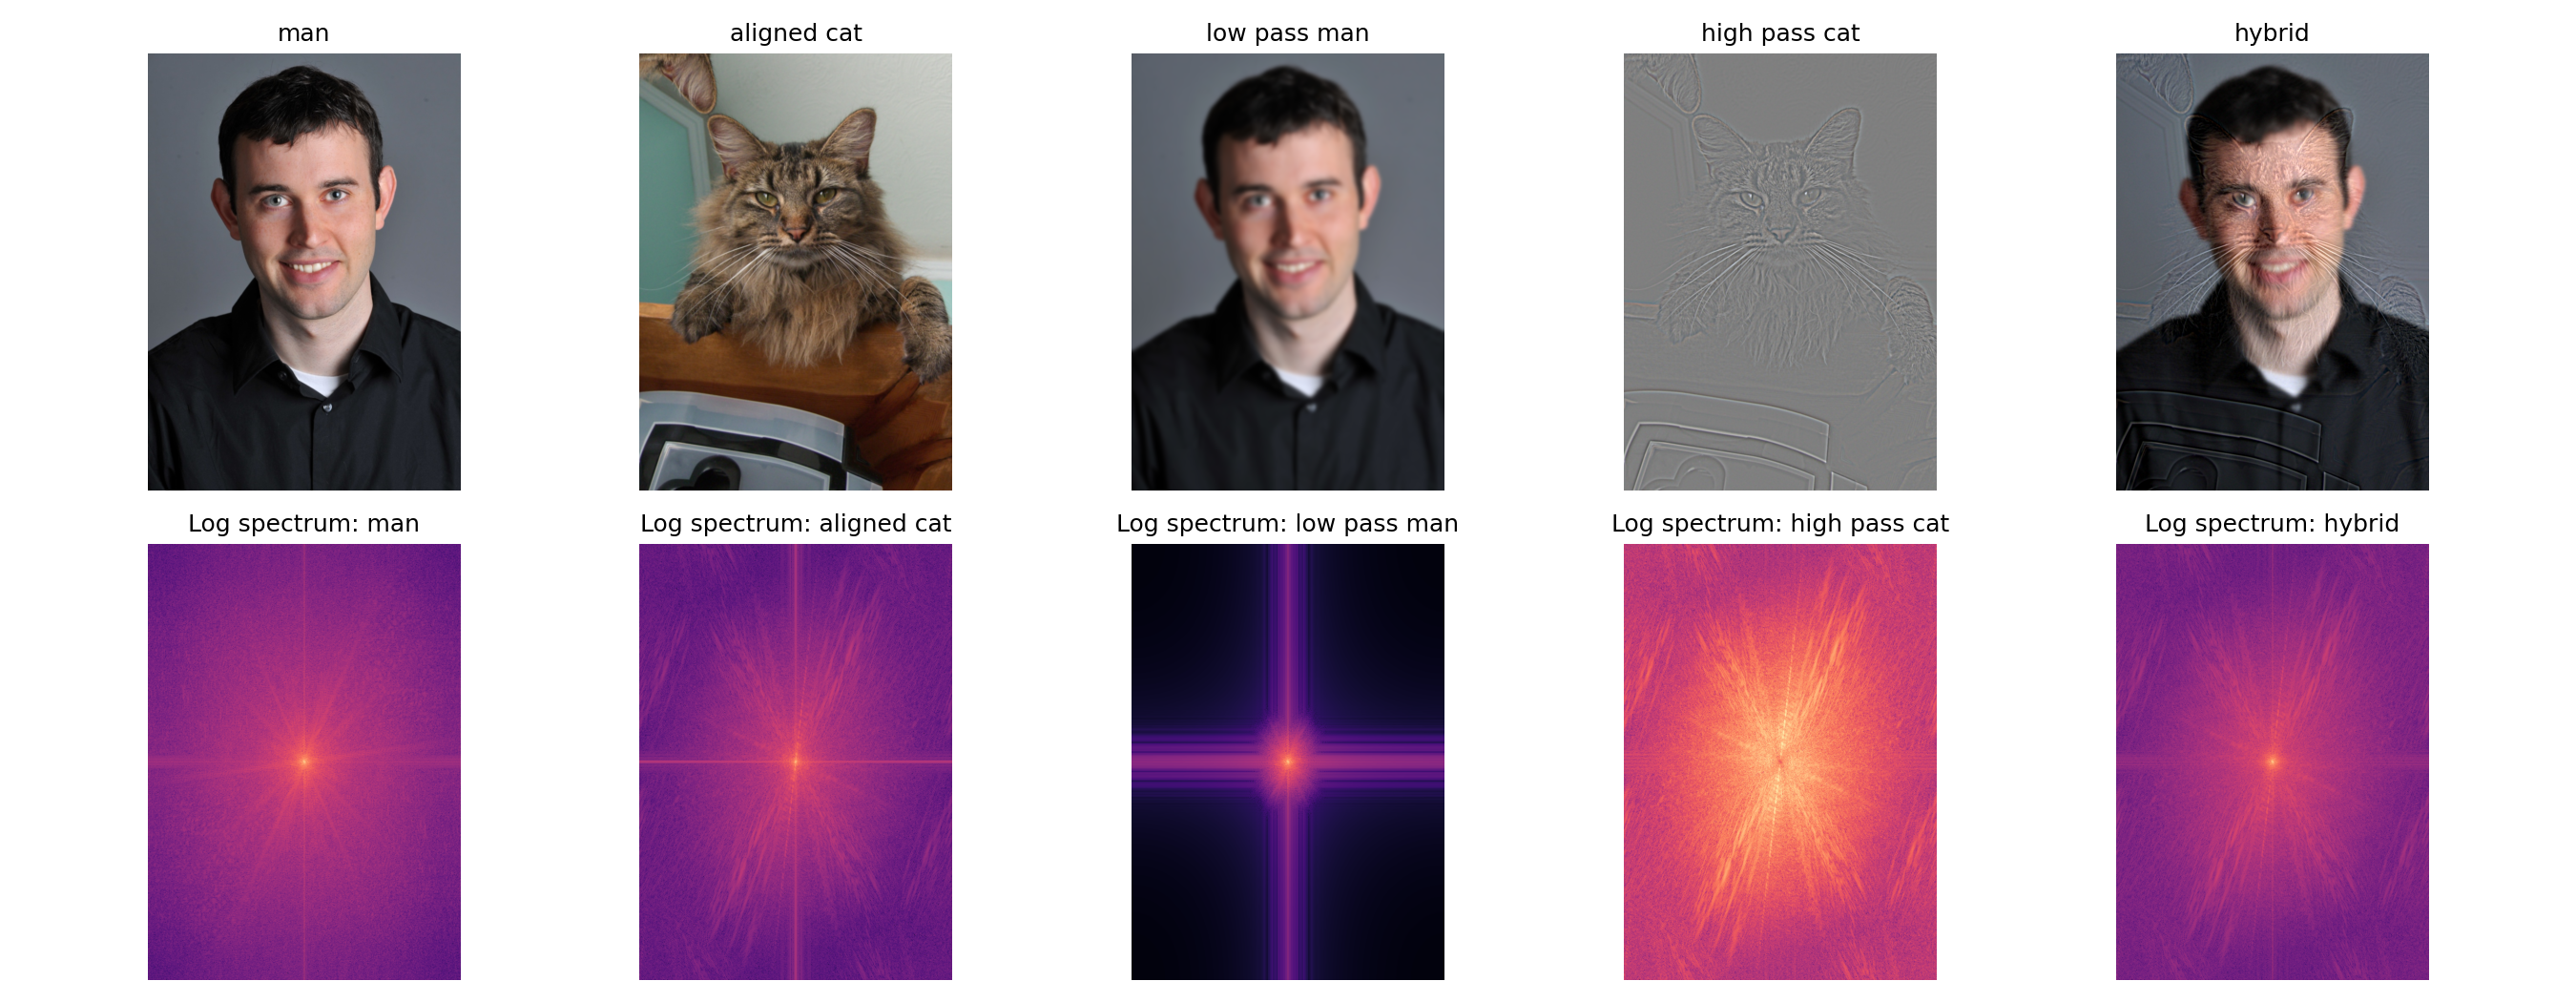
\includegraphics[width=0.97\textwidth]{image_and_spectrum_comparison.png}
  \caption{Combined image-and-spectrum overview for the favourite pair (man--cat).
    Top row: spatial images; bottom row: corresponding log-magnitude spectra.}
  \label{fig:combo}
\end{figure}

%%-----------------------------------------------------------
\subsection{Part 2.2 \texorpdfstring{---}{-} Aliasing and Gaussian Pre-Filtering}
\label{sec:22}
%%-----------------------------------------------------------

\subsubsection{Method}

The Nyquist--Shannon sampling theorem states that downsampling by a factor
of $k$ requires all spatial frequencies above $\pi/k$ to be removed first.
Retaining them causes \emph{aliasing}: high-frequency content folds into
false lower-frequency patterns.

The experiment uses the concentric-rings test image \texttt{rings.png}
($512\times512$ px).  Rings of increasing spatial frequency move from
centre to edge; those near the edge exceed the Nyquist limit of the
$4\times$ downsampled output ($128\times128$) and alias into conspicuous
false rings.

Two strategies are compared:
\begin{enumerate}
  \item \textbf{Direct downsampling:} keep every 4th row and column with no
    pre-filter; implemented in \texttt{aliasing.py} as
    \texttt{downsample\_by\_factor(image, factor=4)}.
  \item \textbf{Gaussian pre-filtering:} apply $G_\sigma$ first, then
    downsample; frequencies above $\pi/4$ are attenuated before sampling.
    Implemented as \texttt{aliasing\_comparison(image, sigma, factor=4)}.
\end{enumerate}

The optimal $\sigma$ is found by a visual sweep over
\[
  \sigma \in \{0.50,\;0.75,\;1.00,\;1.25,\;1.50,\;1.75,\;1.80,\;1.85,\;1.90,\;1.95,\;2.00,\;2.25\}.
\]

\subsubsection{Results}

\begin{figure}[H]
  \centering
  \begin{subfigure}[b]{0.48\textwidth}
    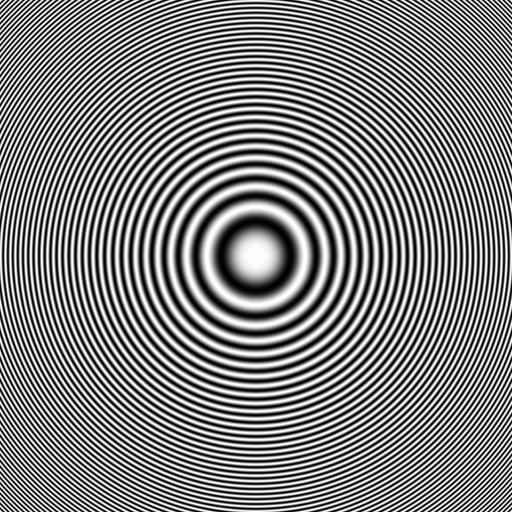
\includegraphics[width=\textwidth]{original.png}
    \caption{Original rings image ($512\times512$).}
  \end{subfigure}\hfill
  \begin{subfigure}[b]{0.48\textwidth}
    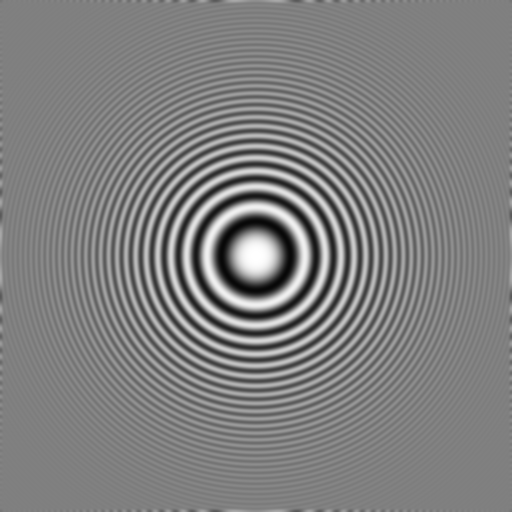
\includegraphics[width=\textwidth]{gaussian_blurred.png}
    \caption{Gaussian-blurred image ($\sigma=2.0$).}
  \end{subfigure}

  \vspace{0.7em}

  \begin{subfigure}[b]{0.48\textwidth}
    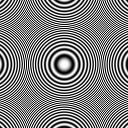
\includegraphics[width=\textwidth]{direct_downsampled.png}
    \caption{\textbf{Direct $4\times$ downsample} ($128\times128$).
      Strong false circles visible in the corners --- aliasing artefacts.}
  \end{subfigure}\hfill
  \begin{subfigure}[b]{0.48\textwidth}
    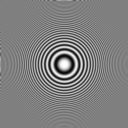
\includegraphics[width=\textwidth]{prefiltered_downsampled.png}
    \caption{\textbf{Pre-filtered then downsampled} ($\sigma=2.0$, $128\times128$).
      Aliasing suppressed; only resolvable rings remain.}
  \end{subfigure}
  \caption{Aliasing comparison on the concentric-rings test image.}
  \label{fig:aliasing_main}
\end{figure}

\begin{figure}[H]
  \centering
  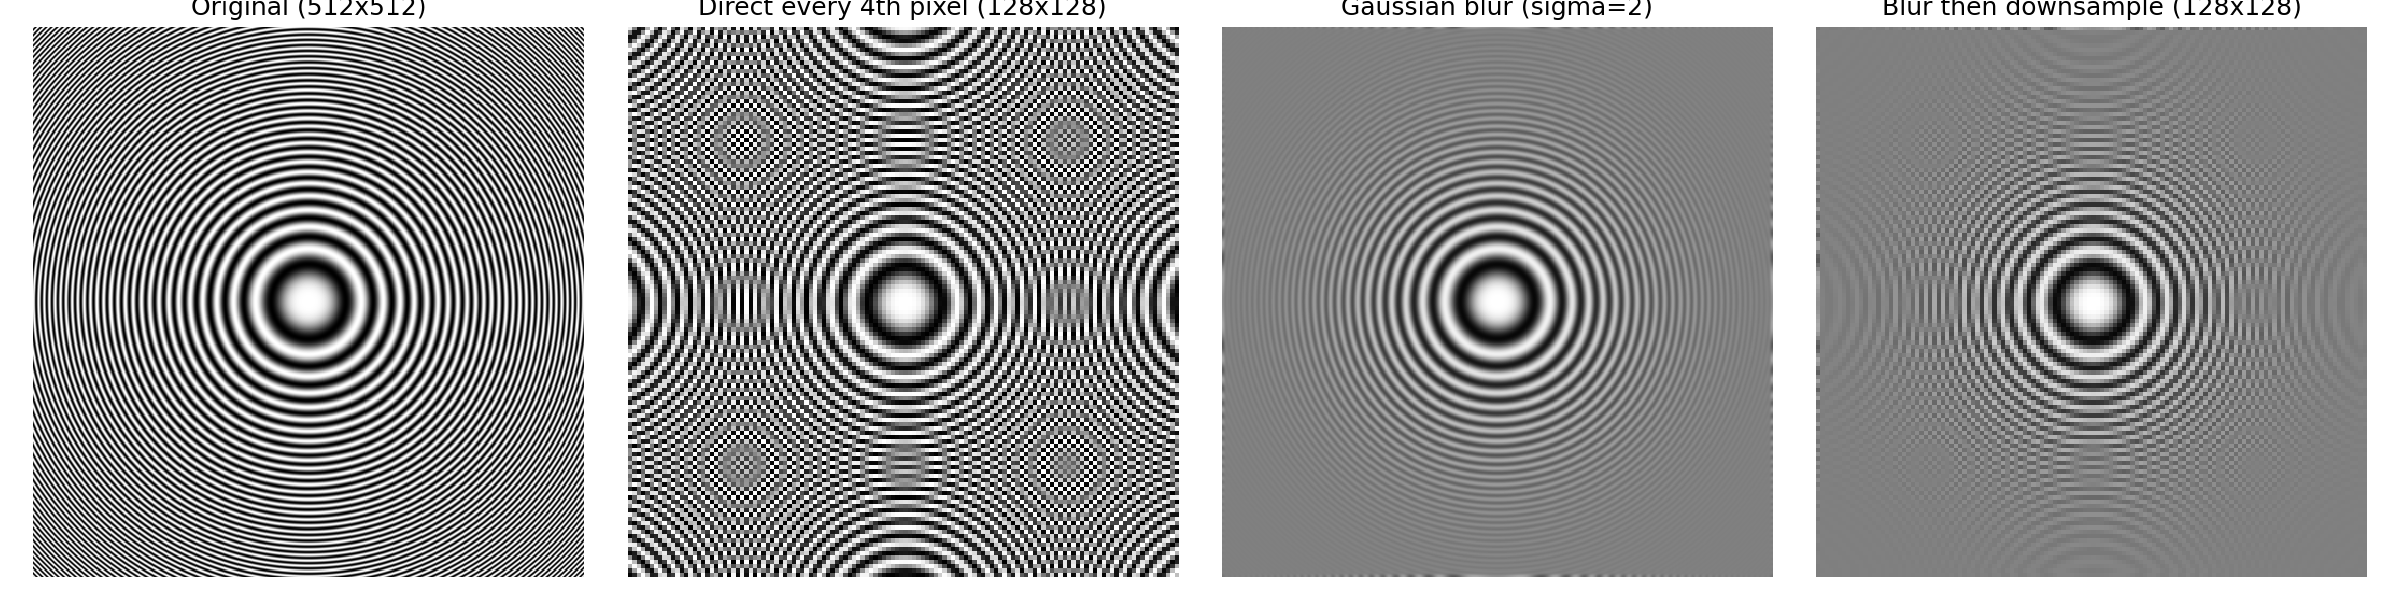
\includegraphics[width=\textwidth]{comparison.png}
  \caption{Three-way side-by-side comparison: original (centre), direct
    downsample (left), and Gaussian pre-filtered downsample (right) displayed
    at the same scale for easy visual comparison.}
  \label{fig:aliasing_comparison}
\end{figure}

\begin{figure}[H]
  \centering
  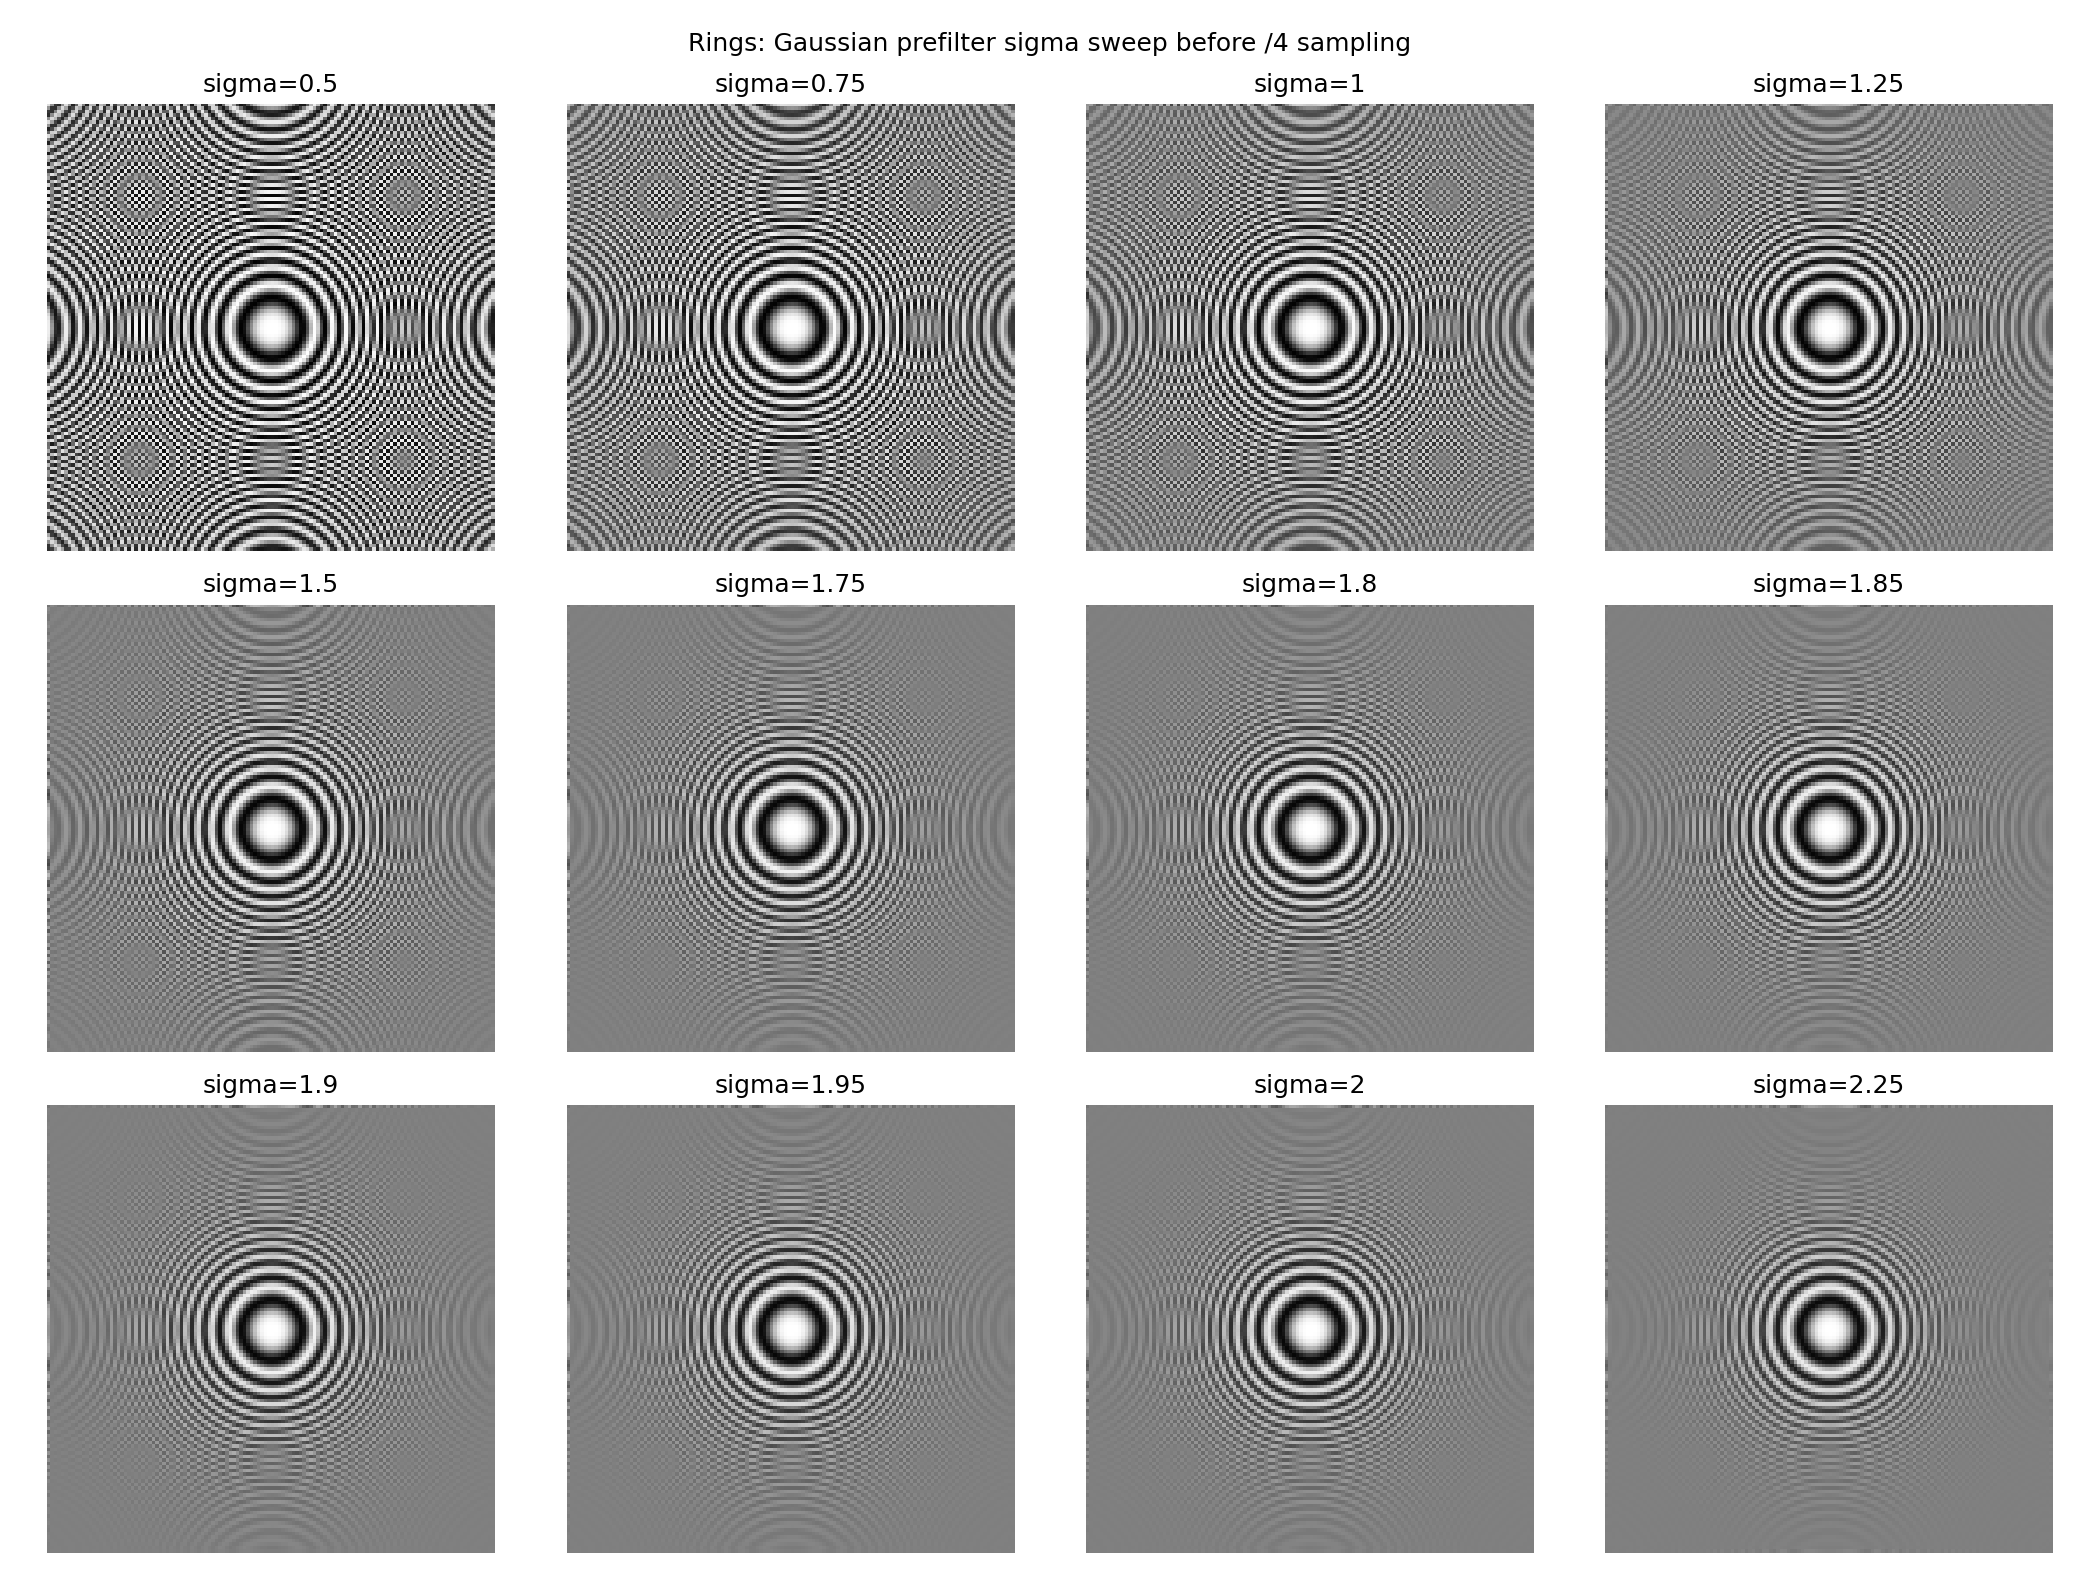
\includegraphics[width=\textwidth]{sigma_sweep.png}
  \caption{Sigma sweep ($\sigma\in\{0.5,\ldots,2.25\}$, $4\times$ downsample).
    False circles gradually disappear as $\sigma$ increases.  At $\sigma=1.95$
    faint residual structure is still visible; at $\sigma=2.0$ it disappears
    at the inspected display scale.}
  \label{fig:sigma_sweep}
\end{figure}

\subsubsection{Discussion}

\textbf{Chosen sigma:} $\boldsymbol{\sigma = 2.0}$ (smallest tested value
without visible false circles).  This is a subjective, image- and
viewing-scale-dependent criterion.

\paragraph{Why aliasing occurs.}
Direct downsampling keeps one sample out of every $4\times4$ block without
removing frequencies above the new Nyquist limit $\pi/4$.  A ring with
spatial frequency $f>\pi/4$ appears in the output at the alias frequency
$|f - \pi/2|$, producing a false ring at a different period.  The result
is the conspicuous false circles visible in Figure~\ref{fig:aliasing_main}(c).

\paragraph{Why Gaussian pre-filtering helps.}
The Gaussian is a low-pass filter; it attenuates energy above its cut-off
frequency before sampling.  With $\sigma=2.0$, energy at $f>\pi/4$ is
negligible by the time the image is sampled, so the alias amplitude is also
negligible.  The pre-filtered output
(Figure~\ref{fig:aliasing_main}(d)) shows only rings resolvable at the output
resolution, with no artefacts.

\paragraph{Connection to Gaussian pyramids.}
Each \texttt{reduce()} step in Part~2.3 applies exactly the same principle:
blur with the binomial filter (a close approximation to a Gaussian) and then
downsample.  This ensures each pyramid level is free of aliasing artefacts
introduced by the coarser sampling grid.

%%-----------------------------------------------------------
\subsection{Part 2.3 \texorpdfstring{---}{-} Gaussian and Laplacian Pyramids}
\label{sec:23}
%%-----------------------------------------------------------

\subsubsection{Method}

\paragraph{Reduce.}
The binomial filter $\mathbf{w} = \tfrac{1}{16}[1,4,6,4,1]$ is applied
separably (horizontally then vertically); every other row and column is kept:
\begin{equation}
  \texttt{reduce}(I) = \bigl(\mathbf{w}\mathbf{w}^\top * I\bigr)[\text{even rows, even cols}].
  \label{eq:reduce}
\end{equation}

\paragraph{Expand.}
Each sample is placed at even row/column positions of a zero-filled grid of
double size; the binomial filter is applied and the result is scaled by 4 to
compensate for the zero-insertion energy loss:
\begin{equation}
  \texttt{expand}(I) = 4\,\bigl(\mathbf{w}\mathbf{w}^\top * I_{\uparrow 2}\bigr).
  \label{eq:expand}
\end{equation}

\paragraph{Gaussian pyramid.}
$G_0 = I$;\quad $G_{k+1} = \texttt{reduce}(G_k)$,
continuing until the smaller side reaches 16 pixels.

\paragraph{Laplacian pyramid.}
\begin{equation}
  L_k = G_k - \texttt{expand}(G_{k+1})[\text{cropped to }G_k\text{'s size}],
  \quad k=0,\ldots,n-2;\qquad
  L_{n-1} = G_{n-1}.
  \label{eq:lap}
\end{equation}
Each $L_k$ stores the detail \emph{not} predicted by the next coarser level.

\paragraph{Reconstruction.}
$R_{n-1} = L_{n-1}$;\quad
$R_k = \texttt{expand}(R_{k+1})[\text{cropped}] + L_k$.
Since $L_k \equiv G_k - \widetilde{G}_{k+1}$, summing recovers $G_k$ exactly
up to floating-point rounding.

\subsubsection{Results}

\textbf{Image:} \texttt{facade.png} ($736\times670$ px ---
\emph{non-power-of-two} dimensions).

\begin{table}[H]
  \centering
  \caption{Gaussian pyramid level dimensions (facade image, min\_size = 16).}
  \label{tab:gpyramid}
  \begin{tabular}{crrr}
    \toprule
    \textbf{Level} & \textbf{Width} & \textbf{Height} & \textbf{Pixels} \\
    \midrule
    0 (original) & 736 & 670 & 493\,120 \\
    1 & 368 & 335 & 123\,280 \\
    2 & 184 & 168 &  30\,912 \\
    3 &  92 &  84 &   7\,728 \\
    4 &  46 &  42 &   1\,932 \\
    5 &  23 &  21 &     483 \\
    6 &  12 &  11 &     132 \\
    \midrule
    \multicolumn{3}{l}{\textbf{Total}} & \textbf{657\,587} \\
    \bottomrule
  \end{tabular}
\end{table}

\textbf{Pixel-count ratio:}
$657\,587 / 493\,120 \approx 1.334$, consistent with the geometric series
$\sum_{k=0}^{\infty}(1/4)^k = 4/3 \approx 1.333$.

\textbf{Reconstruction error:}
Mean absolute error $= 7.67\times10^{-20}$;
maximum absolute error $= 2.22\times10^{-16}$ (machine-precision rounding only).

\begin{figure}[H]
  \centering
  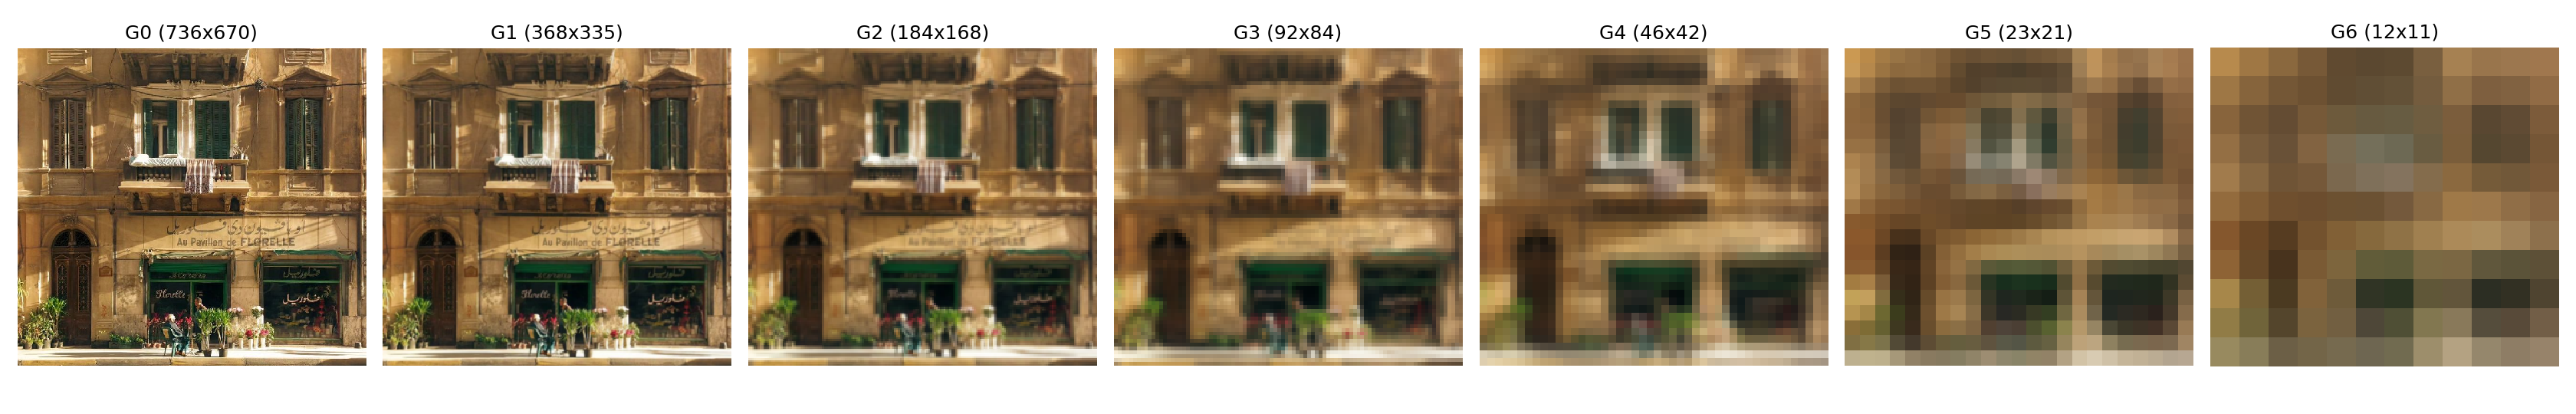
\includegraphics[width=\textwidth]{gaussian_pyramid.png}
  \caption{Full Gaussian pyramid (7 levels, arranged largest to smallest).
    Each successive level is blurred and half-sized in both dimensions.}
  \label{fig:gpyramid}
\end{figure}

\begin{figure}[H]
  \centering
  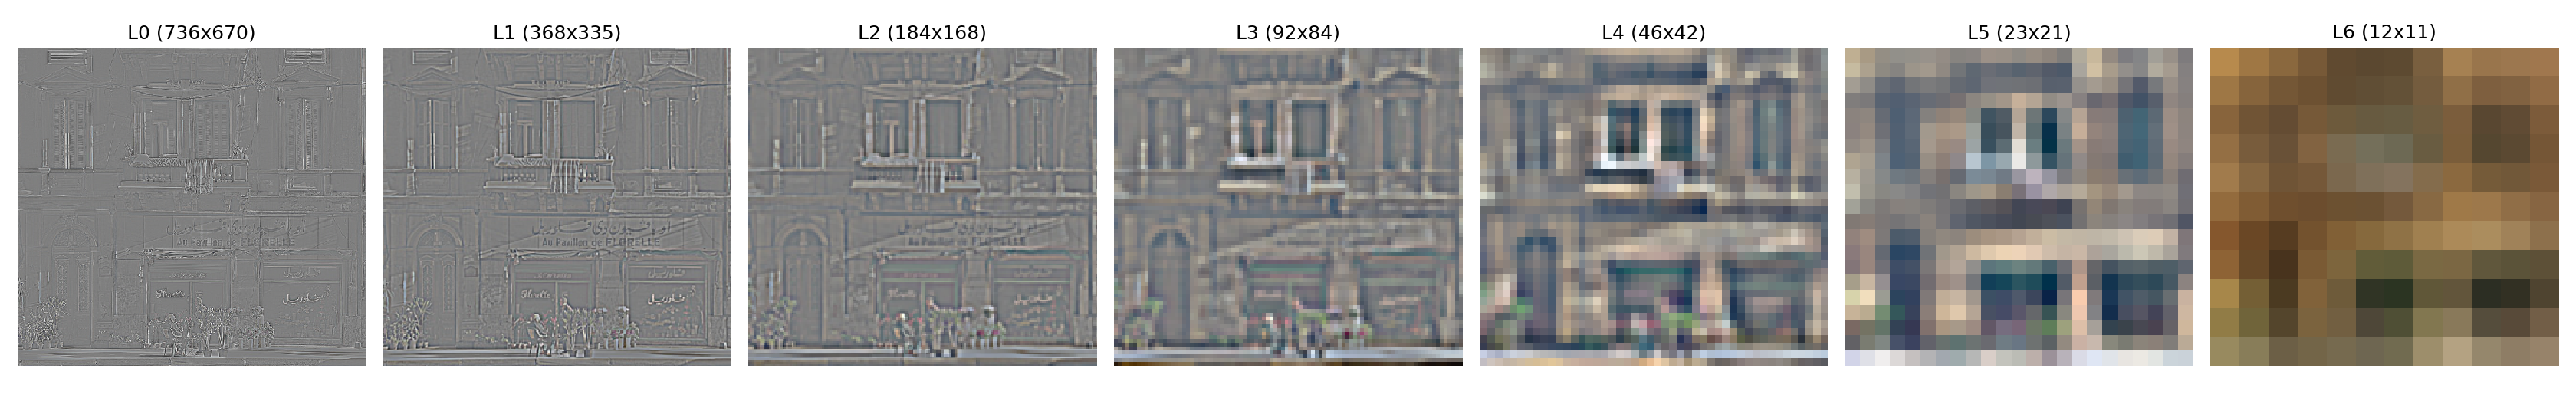
\includegraphics[width=\textwidth]{laplacian_pyramid.png}
  \caption{Full Laplacian pyramid.  Each level stores a band-pass residual
    $L_k = G_k - \texttt{expand}(G_{k+1})$; the final level is the coarsest
    Gaussian.  Values are shifted to $[0,255]$ for display.}
  \label{fig:lpyramid}
\end{figure}

\begin{figure}[H]
  \centering
  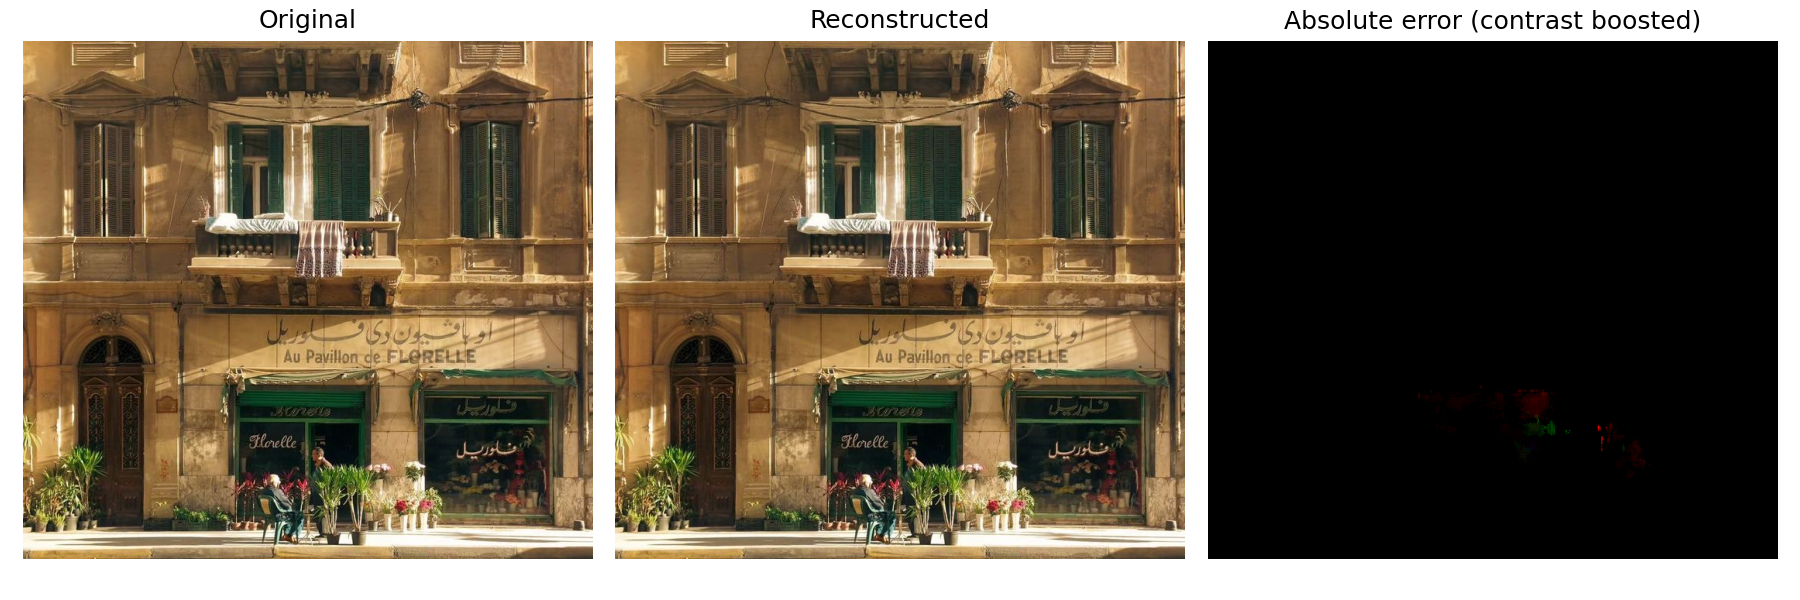
\includegraphics[width=0.88\textwidth]{reconstruction_comparison.png}
  \caption{Left: original image; centre: reconstructed image;
    right: contrast-boosted absolute error
    (scaled by $2.22\times10^{-16}$).
    The error is at machine precision --- reconstruction is effectively exact.}
  \label{fig:reconstruction}
\end{figure}

\subsubsection{Individual Pyramid Levels}

\begin{figure}[H]
  \centering
  \begin{subfigure}[b]{0.30\textwidth}
    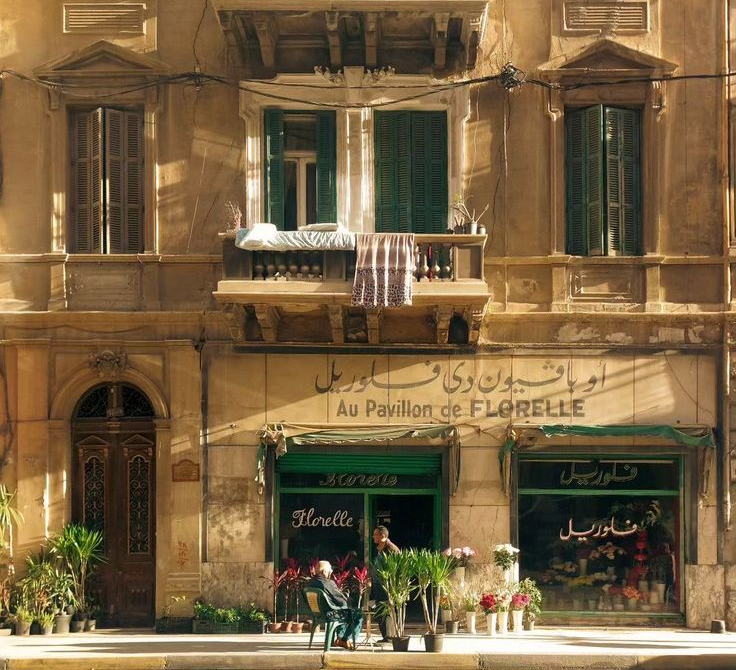
\includegraphics[width=\textwidth]{outputs/part2_3/gaussian_pyramid/level_00.png}
    \caption{$G_0$: 736$\times$670.}
  \end{subfigure}\hfill
  \begin{subfigure}[b]{0.22\textwidth}
    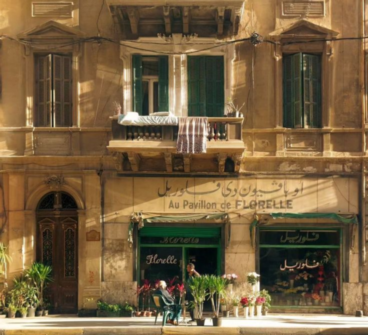
\includegraphics[width=\textwidth]{outputs/part2_3/gaussian_pyramid/level_01.png}
    \caption{$G_1$: 368$\times$335.}
  \end{subfigure}\hfill
  \begin{subfigure}[b]{0.14\textwidth}
    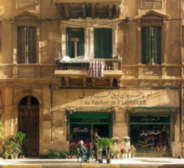
\includegraphics[width=\textwidth]{outputs/part2_3/gaussian_pyramid/level_02.png}
    \caption{$G_2$: 184$\times$168.}
  \end{subfigure}\hfill
  \begin{subfigure}[b]{0.10\textwidth}
    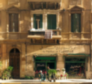
\includegraphics[width=\textwidth]{outputs/part2_3/gaussian_pyramid/level_03.png}
    \caption{$G_3$.}
  \end{subfigure}
  \caption{Gaussian pyramid levels 0--3; spatial detail decreases with level.}
  \label{fig:glevels}
\end{figure}

\begin{figure}[H]
  \centering
  \begin{subfigure}[b]{0.30\textwidth}
    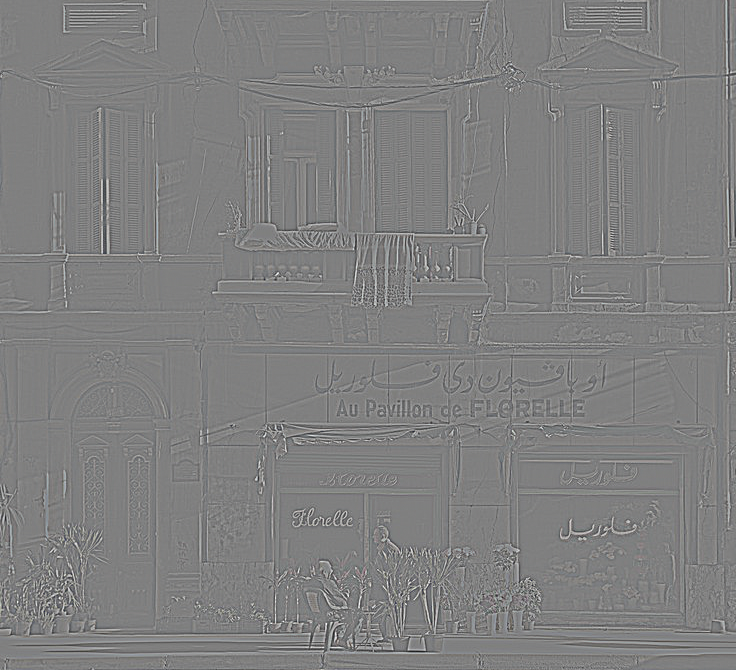
\includegraphics[width=\textwidth]{outputs/part2_3/laplacian_pyramid/level_00.png}
    \caption{$L_0$: fine edges \& texture.}
  \end{subfigure}\hfill
  \begin{subfigure}[b]{0.22\textwidth}
    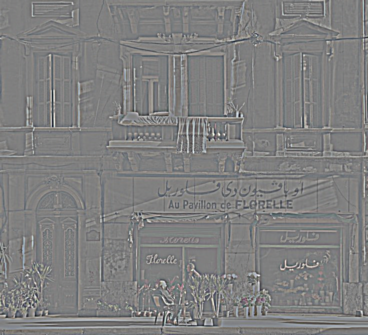
\includegraphics[width=\textwidth]{outputs/part2_3/laplacian_pyramid/level_01.png}
    \caption{$L_1$: medium detail.}
  \end{subfigure}\hfill
  \begin{subfigure}[b]{0.14\textwidth}
    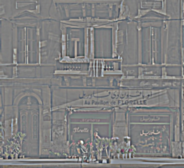
\includegraphics[width=\textwidth]{outputs/part2_3/laplacian_pyramid/level_02.png}
    \caption{$L_2$: coarser detail.}
  \end{subfigure}\hfill
  \begin{subfigure}[b]{0.10\textwidth}
    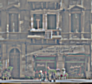
\includegraphics[width=\textwidth]{outputs/part2_3/laplacian_pyramid/level_03.png}
    \caption{$L_3$.}
  \end{subfigure}
  \caption{Laplacian pyramid levels 0--3 (display-normalised).
    $L_0$ holds the finest details; each higher index captures a progressively
    coarser spatial-frequency band.}
  \label{fig:llevels}
\end{figure}

\subsubsection{Discussion}

\paragraph{Why reconstruction is exact.}
Each level $L_k = G_k - \widetilde{G}_{k+1}$ stores exactly the difference
between the Gaussian level and its reconstruction predictor
$\widetilde{G}_{k+1} = \texttt{expand}(G_{k+1})[\text{cropped}]$.
Summing $\widetilde{G}_{k+1} + L_k$ recovers $G_k$ algebraically; the only
residual error is 64-bit floating-point rounding (MAE $<10^{-19}$).

\paragraph{Why the lecture's blur-residual version is not exact.}
The lecture version subtracts a level's \emph{own} blurred copy:
$L_k^{\text{lec}} = G_k - \mathrm{blur}(G_k)$.
This residual \emph{cannot} be used to recover $G_k$ from $G_{k+1}$ because
$\widetilde{G}_{k+1} \neq \mathrm{blur}(G_k)$ in general, so
$\widetilde{G}_{k+1} + L_k^{\text{lec}} \neq G_k$.

\paragraph{Handling odd dimensions.}
When $G_k$ has odd width $w$, \texttt{expand}($G_{k+1}$) produces $w-1$ or
$w+1$ columns depending on the direction of rounding.  Only the trailing
row/column is cropped; no internal pixels are discarded, and the reconstruction
identity is preserved.

\paragraph{Pixel-count ratio.}
Levels at depth $k$ contain $\approx(1/4)^k$ of the original pixels,
giving a total that converges to
$N\sum_{k=0}^{\infty}(1/4)^k = \tfrac{4}{3}N \approx 1.333N$.
The measured value 1.334 reflects the finite pyramid depth and ceil-halving
of the odd-dimensioned facade.

%%-----------------------------------------------------------
\subsection{Part 2.4 \texorpdfstring{---}{-} Multiresolution Image Blending}
\label{sec:24}
%%-----------------------------------------------------------

\subsubsection{Method}

Multiresolution (Laplacian) blending \cite{BurtAdelson1983} avoids seam
artefacts by blending each frequency band of the Laplacian pyramid separately,
using a mask that is \emph{smoothed to match the band's spatial scale}:

\begin{equation}
  B_k = M_k \cdot L_k^{(1)} + (1 - M_k) \cdot L_k^{(2)},
  \label{eq:blend}
\end{equation}

where $M_k$ is level $k$ of the \textbf{Gaussian pyramid} of the binary mask,
$L_k^{(1)}, L_k^{(2)}$ are the Laplacian pyramids of the two source images,
and $B_k$ is the blended Laplacian band.  The blended image is then
reconstructed from $\{B_k\}$.

At the finest level ($k=0$), $M_0$ is close to the original binary mask,
giving a sharp seam.  At coarser levels, $M_k$ is heavily Gaussian-blurred
and the seam transitions over a wide area — matched to the coarser spatial
wavelength of that band.  The result hides the seam at \emph{every} frequency.

\textbf{Implementation} (\texttt{blending.py}):
\texttt{build\_blended\_laplacian\_pyramid} constructs $L^{(1)}$, $L^{(2)}$,
and the mask Gaussian pyramid; \texttt{multiresolution\_blend} wraps it and
calls \texttt{reconstruct\_from\_laplacian}.

\subsubsection{Blend 1 \texorpdfstring{---}{-} Apple / Orange (Classic Example)}

\textbf{Mask:} Vertical half-plane (left half selects apple, right half
selects orange).
\textbf{Pyramid:} 6 levels, $512\times512$ down to $16\times16$.

\begin{figure}[H]
  \centering
  \begin{subfigure}[b]{0.22\textwidth}
    \includegraphics[width=\textwidth]{outputs/part2_4/apple-orange/first_image.png}
    \caption{Apple.}
  \end{subfigure}\hfill
  \begin{subfigure}[b]{0.22\textwidth}
    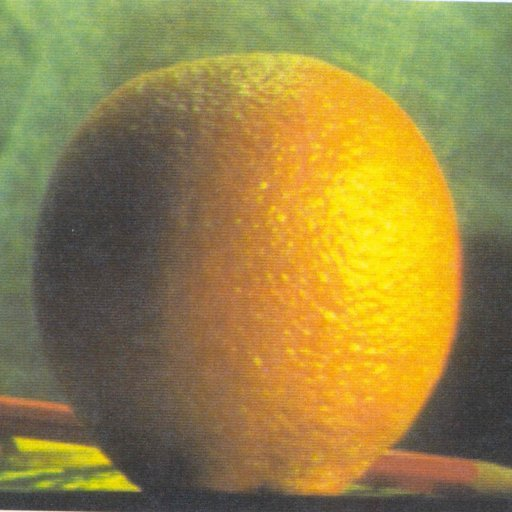
\includegraphics[width=\textwidth]{outputs/part2_4/apple-orange/second_image.png}
    \caption{Orange.}
  \end{subfigure}\hfill
  \begin{subfigure}[b]{0.22\textwidth}
    
\includegraphics[width=\textwidth]{outputs/part2_4/apple-orange/mask.png}
    \caption{Binary mask.}
  \end{subfigure}\hfill
  \begin{subfigure}[b]{0.22\textwidth}
    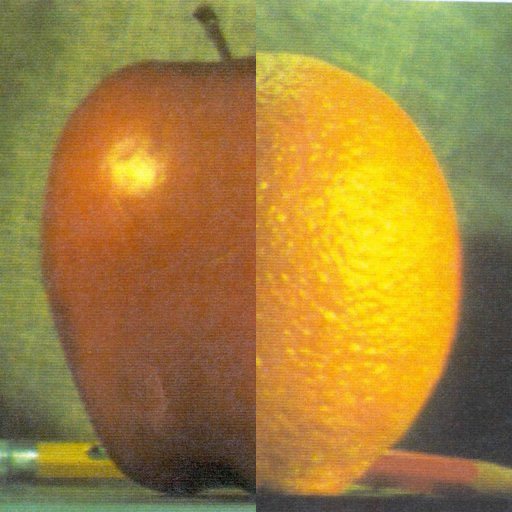
\includegraphics[width=\textwidth]{outputs/part2_4/apple-orange/hard_cut.png}
    \caption{Hard cut.}
  \end{subfigure}
  \caption{Apple--Orange inputs, mask, and naive hard cut.}
  \label{fig:ao_inputs}
\end{figure}

\begin{figure}[H]
  \centering
  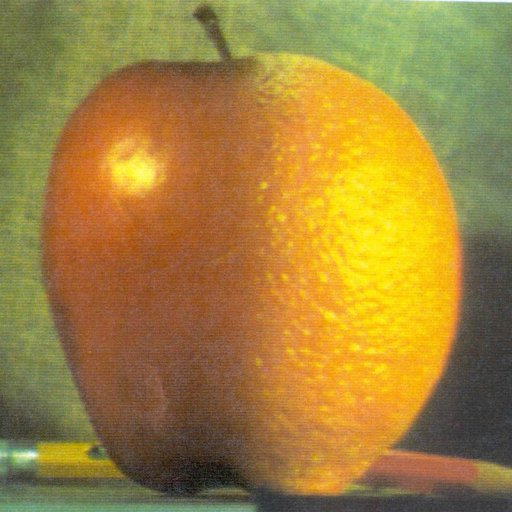
\includegraphics[width=0.55\textwidth]{outputs/part2_4/apple-orange/blended.png}
  \caption{Apple--Orange \textbf{multiresolution blend}.
    The seam is invisible; colour and texture transition smoothly.}
  \label{fig:ao_blend}
\end{figure}

\begin{figure}[H]
  \centering
  \begin{subfigure}[b]{0.48\textwidth}
    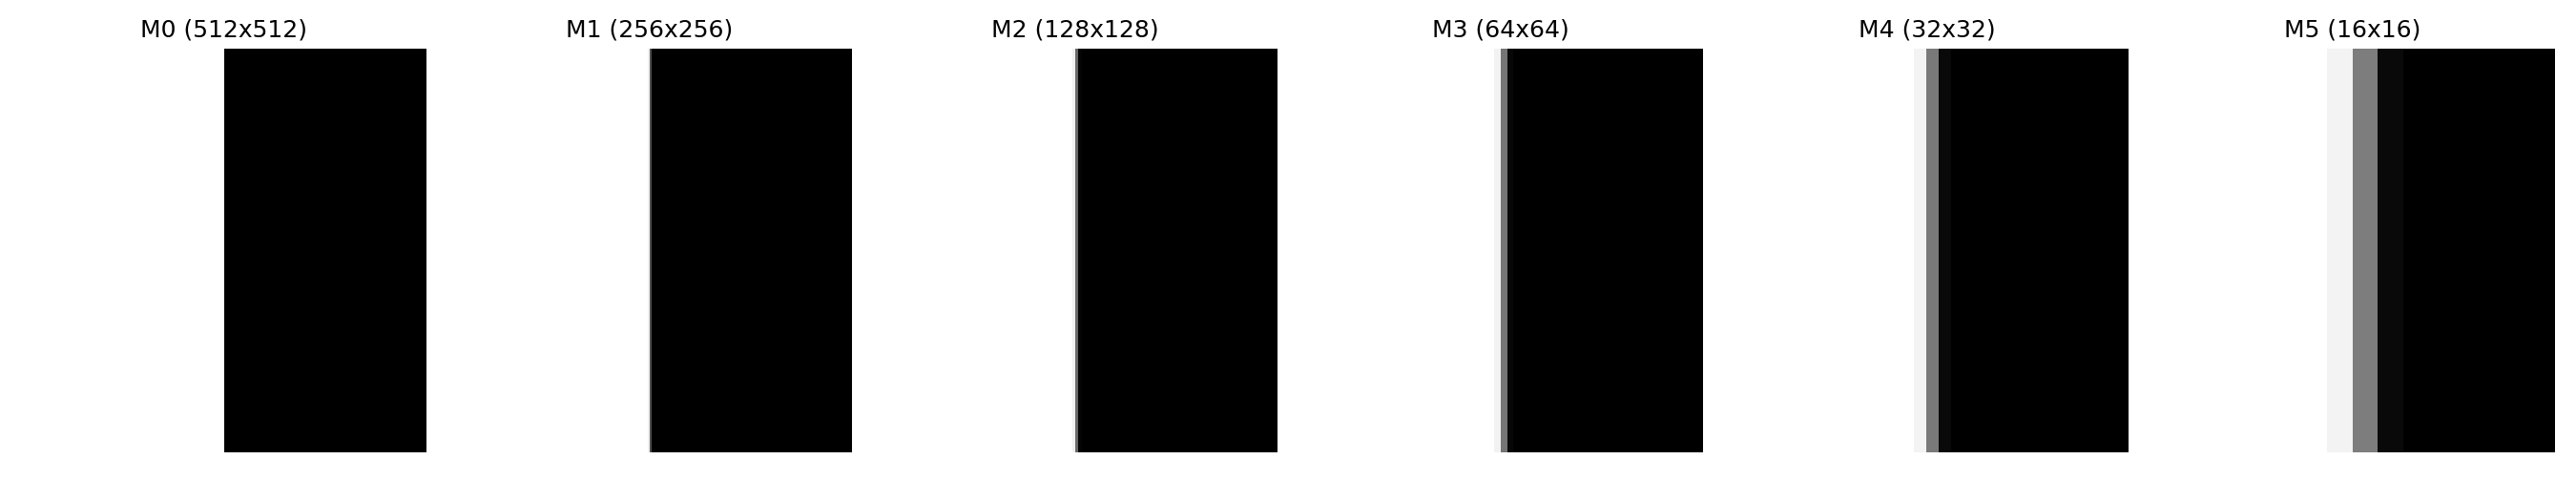
\includegraphics[width=\textwidth]{outputs/part2_4/apple-orange/mask_gaussian_pyramid.png}
    \caption{Mask Gaussian pyramid (transition widens with level).}
  \end{subfigure}\hfill
  \begin{subfigure}[b]{0.48\textwidth}
    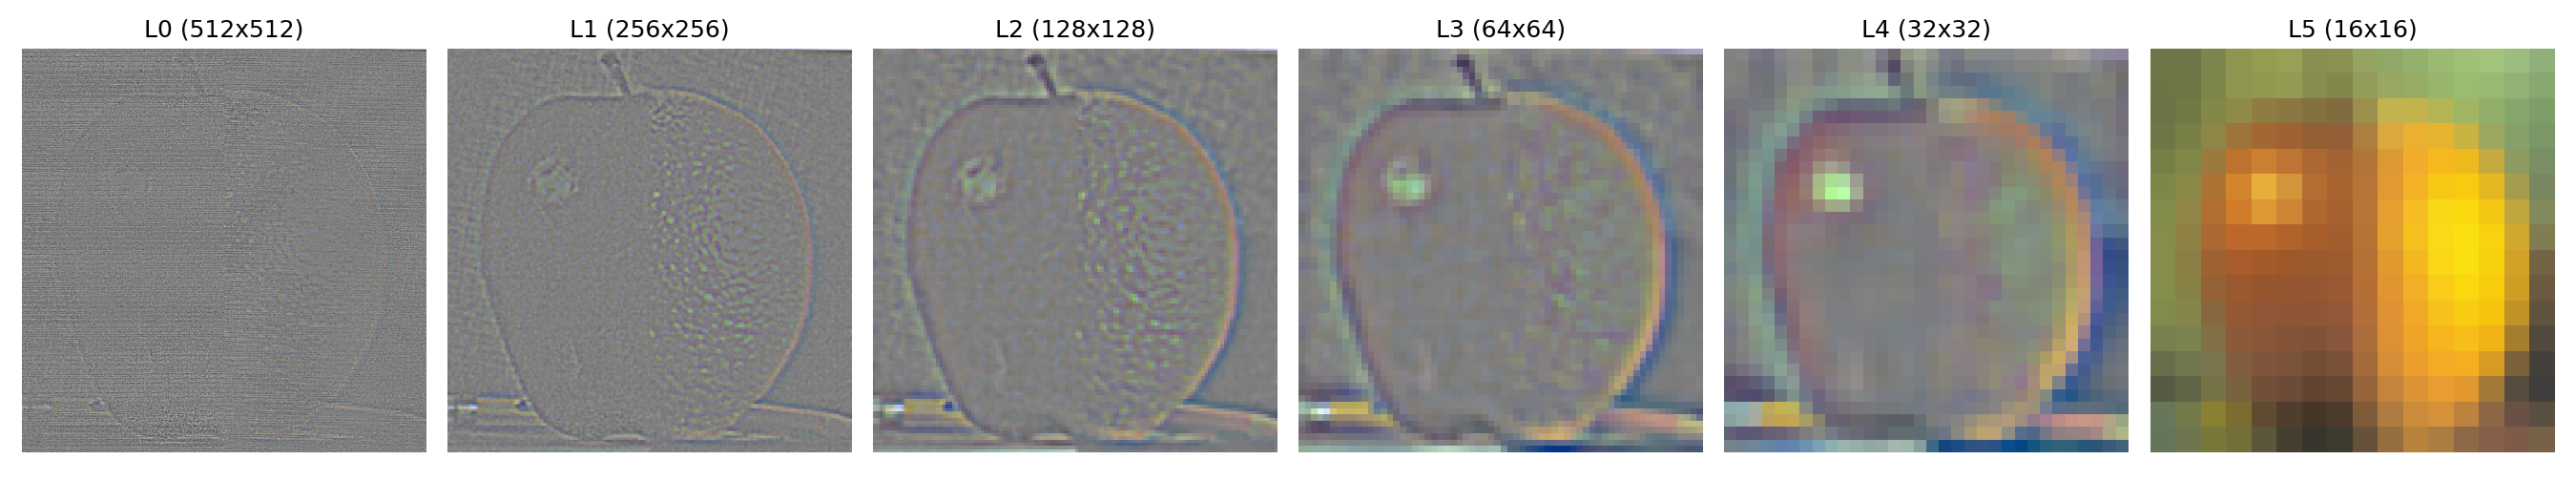
\includegraphics[width=\textwidth]{outputs/part2_4/apple-orange/blended_laplacian_pyramid.png}
    \caption{Blended Laplacian pyramid ($B_k$ at each level).}
  \end{subfigure}
  \caption{Apple--Orange pyramid analysis.}
  \label{fig:ao_pyr}
\end{figure}

\begin{figure}[H]
  \centering
  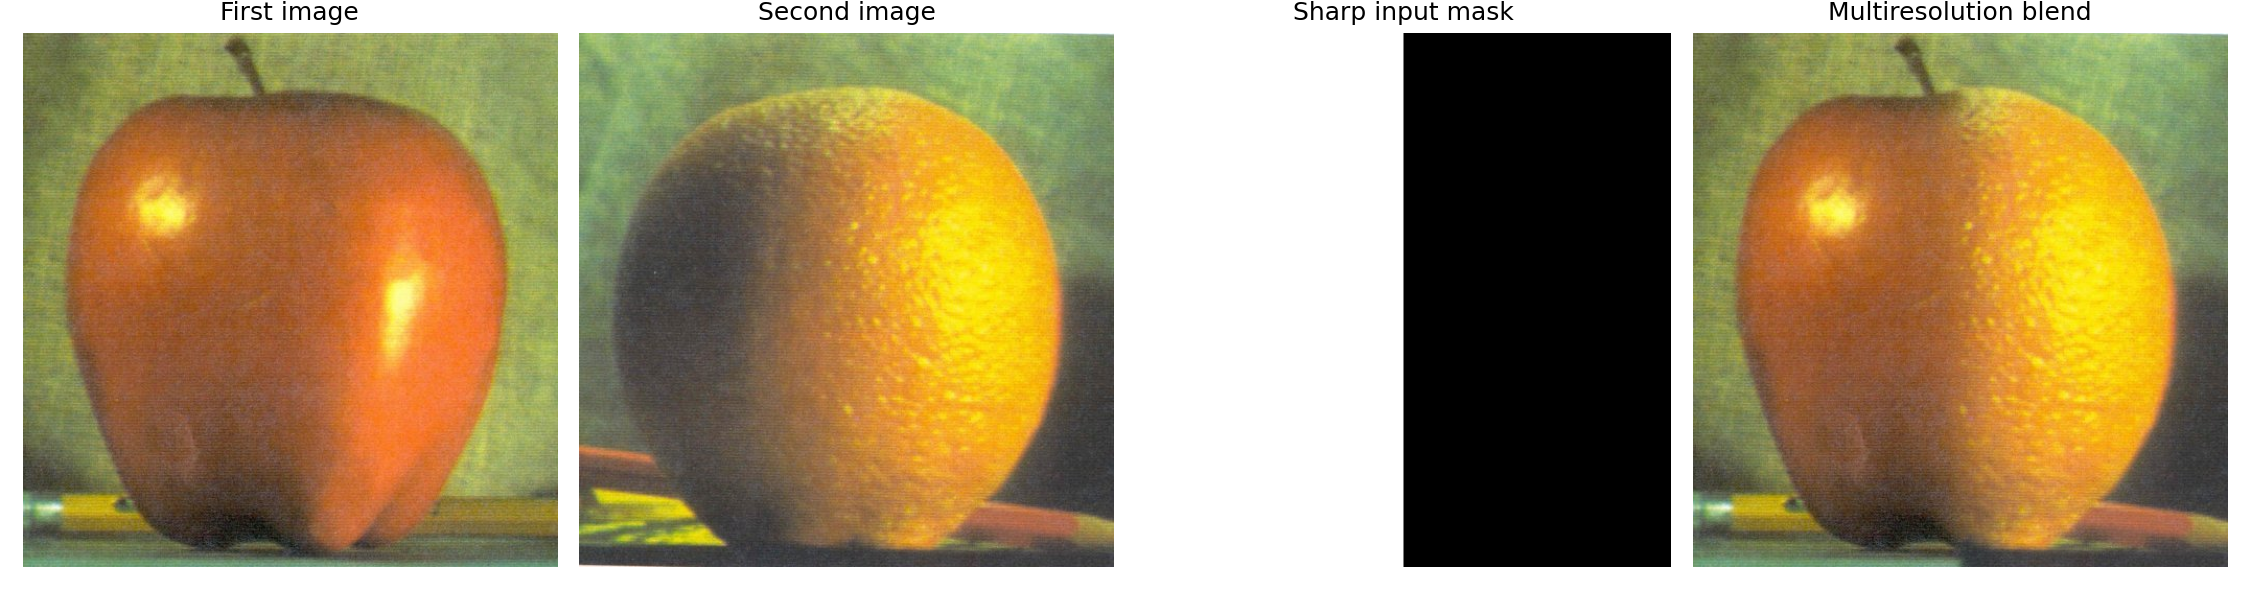
\includegraphics[width=\textwidth]{outputs/part2_4/apple-orange/comparison.png}
  \caption{Apple--Orange full comparison: hard cut (left) vs.\ blend (right).}
  \label{fig:ao_cmp}
\end{figure}

\subsubsection{Blend 2 \texorpdfstring{---}{-} Eye on Hand}

\textbf{Mask:} Binary ellipse centred on the palm.
\textbf{Pyramid:} 7 levels, $900\times675$ down to $15\times11$.
The eye is aligned to the palm using README-provided landmark points.

\begin{figure}[H]
  \centering
  \begin{subfigure}[b]{0.22\textwidth}
    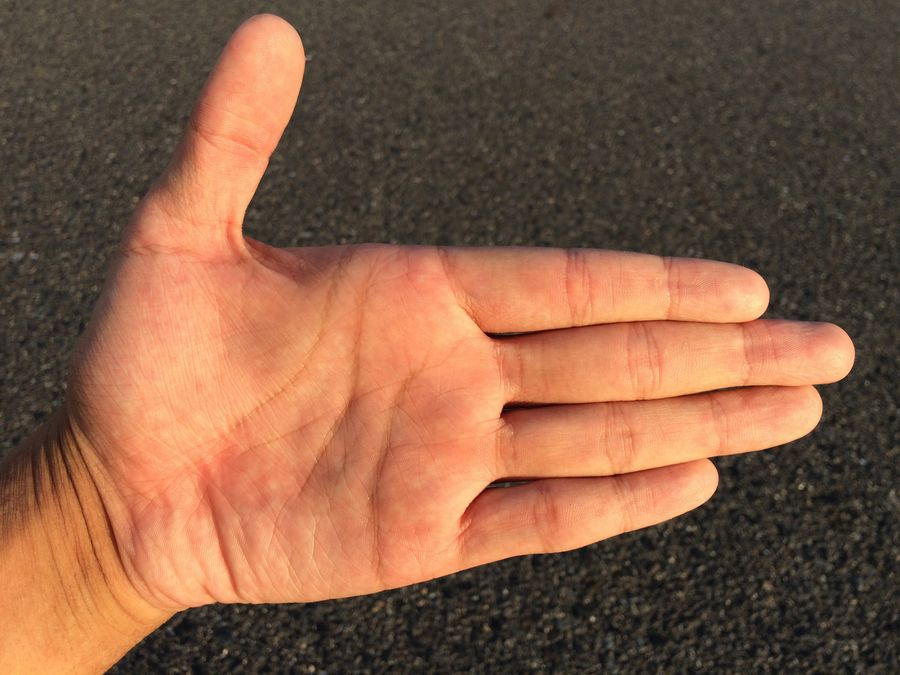
\includegraphics[width=\textwidth]{outputs/part2_4/eye-on-hand/first_image.png}
    \caption{Eye image.}
  \end{subfigure}\hfill
  \begin{subfigure}[b]{0.22\textwidth}
    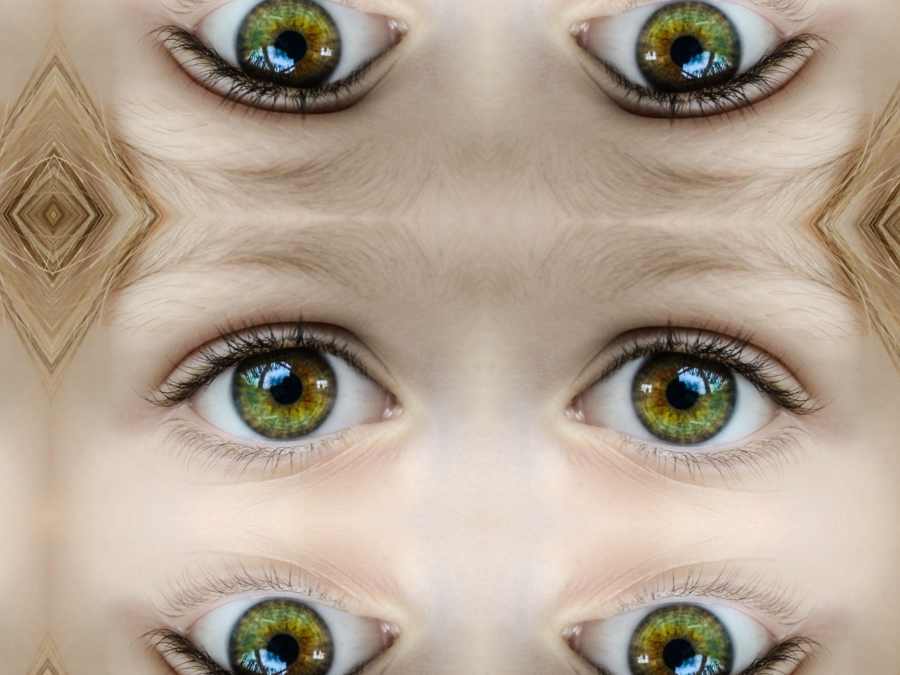
\includegraphics[width=\textwidth]{outputs/part2_4/eye-on-hand/second_image.png}
    \caption{Hand image.}
  \end{subfigure}\hfill
  \begin{subfigure}[b]{0.22\textwidth}
    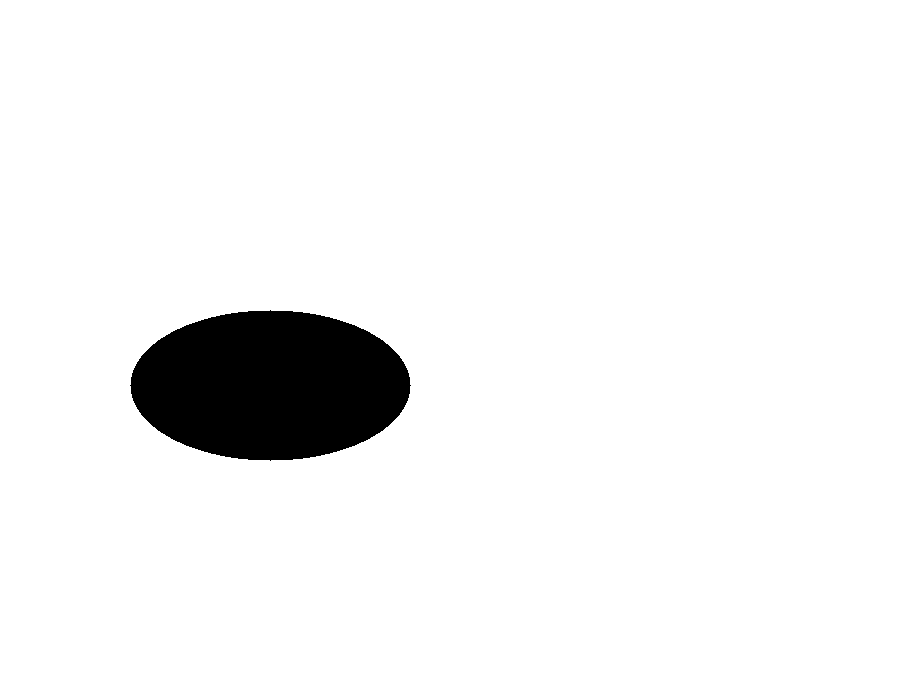
\includegraphics[width=\textwidth]{outputs/part2_4/eye-on-hand/mask.png}
    \caption{Elliptical mask.}
  \end{subfigure}\hfill
  \begin{subfigure}[b]{0.22\textwidth}
    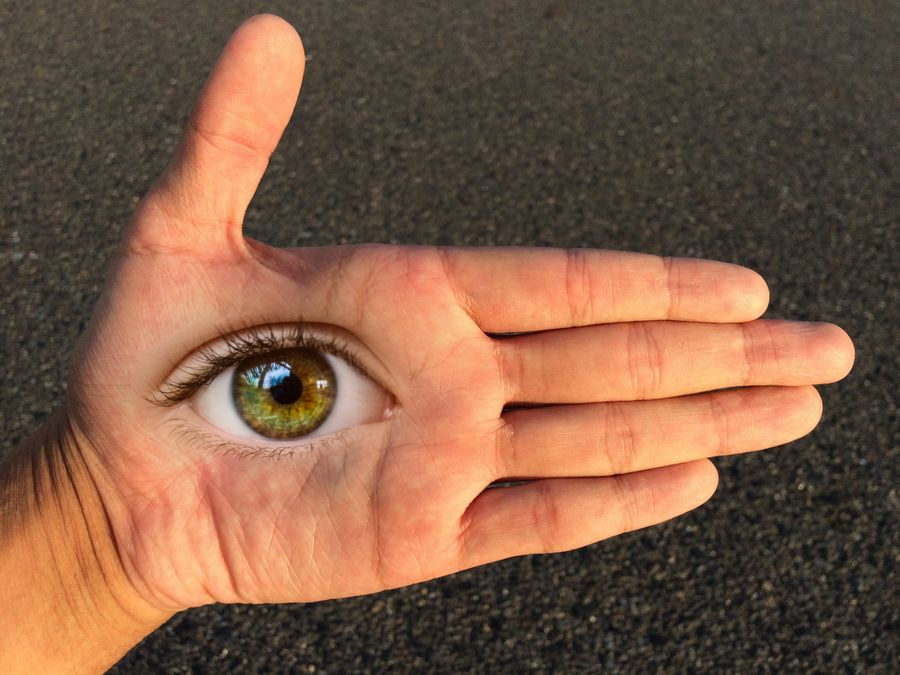
\includegraphics[width=\textwidth]{outputs/part2_4/eye-on-hand/blended.png}
    \caption{Blended.}
  \end{subfigure}
  \caption{\textbf{Eye-on-Hand blend.}  The elliptical mask places the eye
    onto the palm; multiresolution blending integrates skin textures seamlessly.}
  \label{fig:eye_blend}
\end{figure}

\begin{figure}[H]
  \centering
  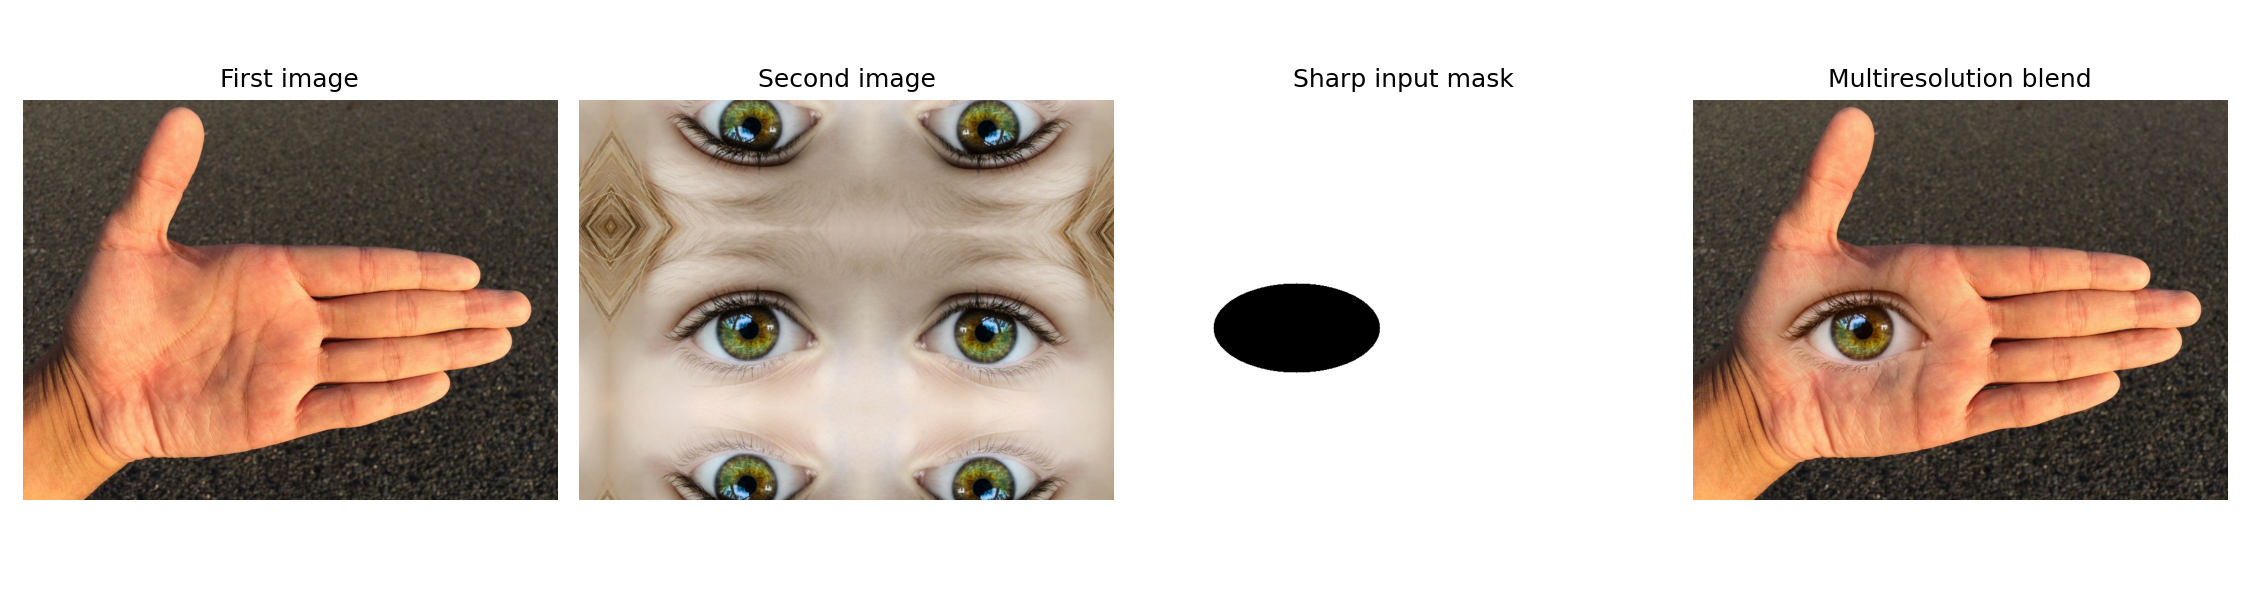
\includegraphics[width=\textwidth]{outputs/part2_4/eye-on-hand/comparison.png}
  \caption{Eye-on-Hand: hard cut (left) vs.\ multiresolution blend (right).}
  \label{fig:eye_cmp}
\end{figure}

\subsubsection{Blend 3 \texorpdfstring{---}{-} Cat on Sunflower}

\textbf{Mask:} Three overlapping ellipses forming a head-and-ears silhouette.
\textbf{Pyramid:} 6 levels, $612\times408$ down to $20\times13$.
Cat eyes are aligned to the sunflower centre.

\begin{figure}[H]
  \centering
  \begin{subfigure}[b]{0.22\textwidth}
    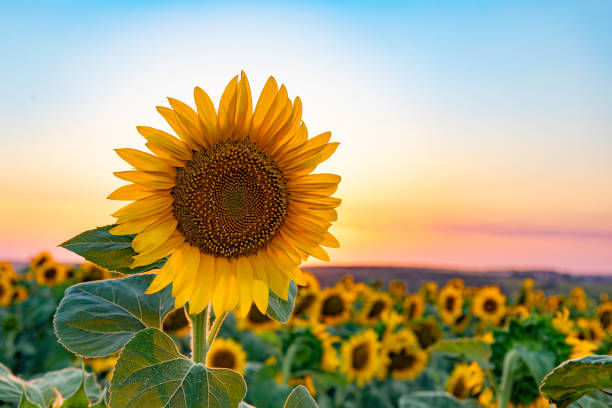
\includegraphics[width=\textwidth]{outputs/part2_4/cat-on-sunflower/first_image.png}
    \caption{Cat.}
  \end{subfigure}\hfill
  \begin{subfigure}[b]{0.22\textwidth}
    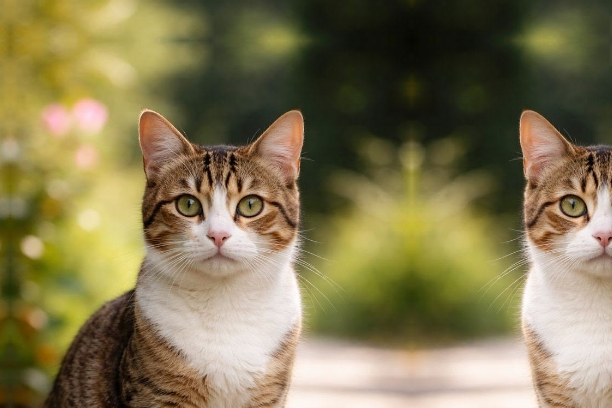
\includegraphics[width=\textwidth]{outputs/part2_4/cat-on-sunflower/second_image.png}
    \caption{Sunflower.}
  \end{subfigure}\hfill
  \begin{subfigure}[b]{0.22\textwidth}
    
\includegraphics[width=\textwidth]{outputs/part2_4/cat-on-sunflower/mask.png}
    \caption{Head-and-ears mask.}
  \end{subfigure}\hfill
  \begin{subfigure}[b]{0.22\textwidth}
    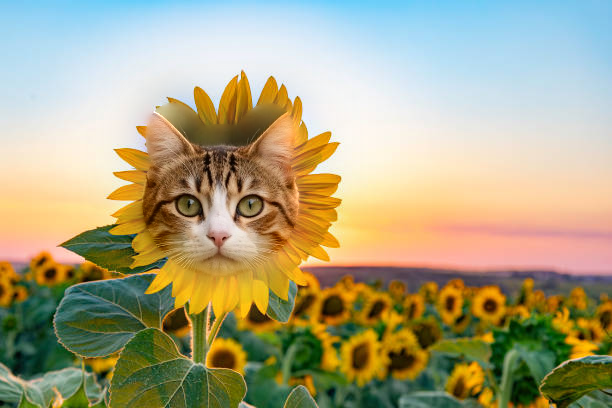
\includegraphics[width=\textwidth]{outputs/part2_4/cat-on-sunflower/blended.png}
    \caption{Blended.}
  \end{subfigure}
  \caption{\textbf{Cat-on-Sunflower blend.}
    The head-and-ears mask composites the cat face onto the sunflower centre;
    petals remain visible around the blend region.}
  \label{fig:cat_blend}
\end{figure}

\begin{figure}[H]
  \centering
  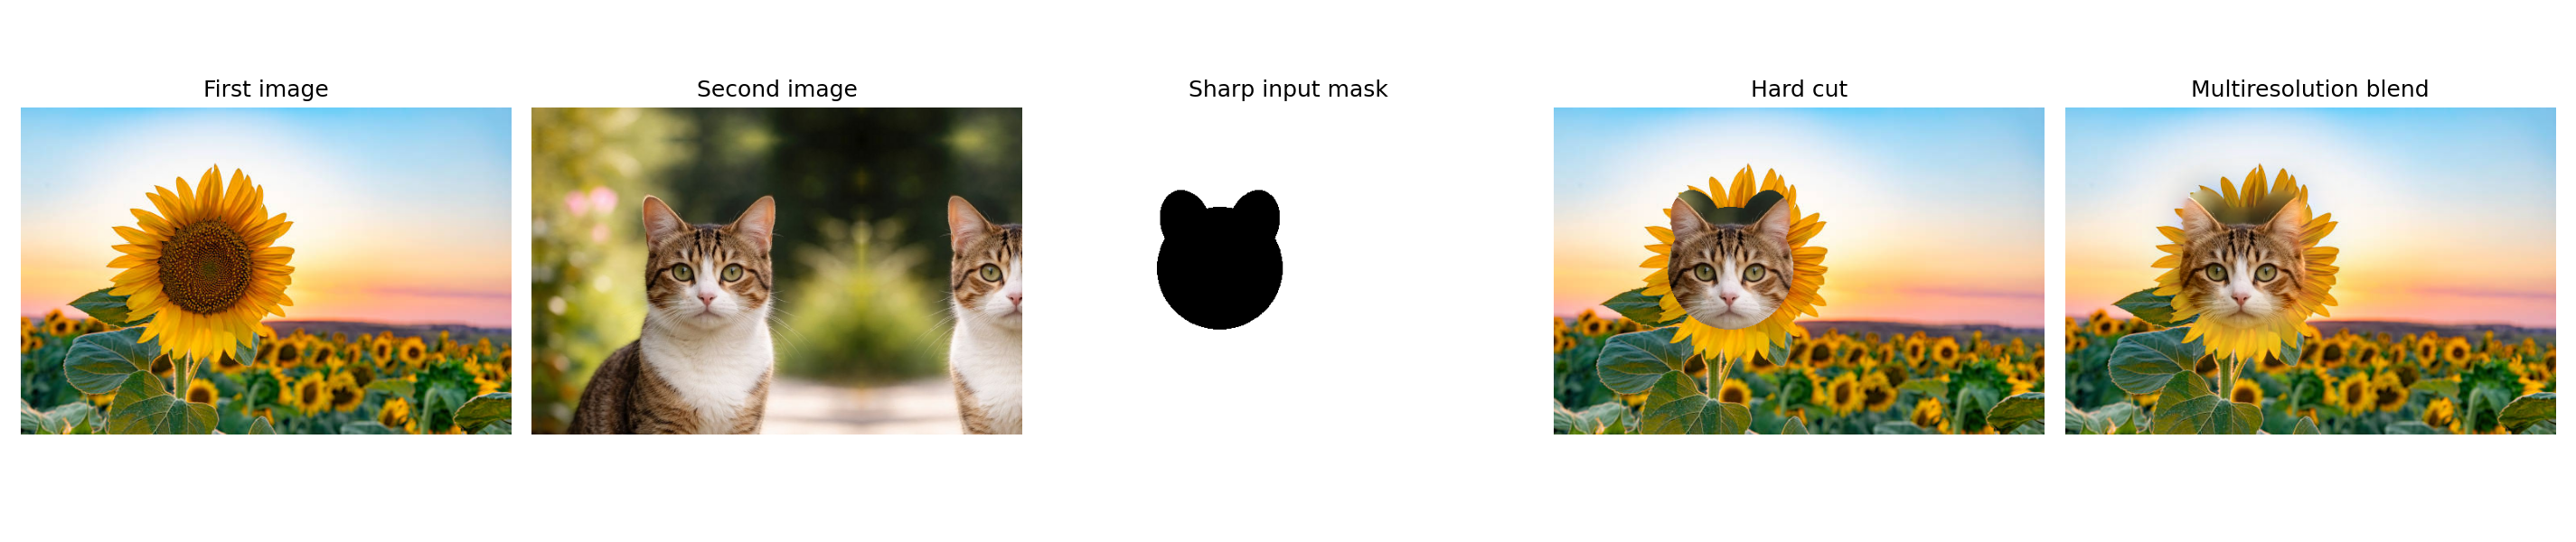
\includegraphics[width=\textwidth]{outputs/part2_4/cat-on-sunflower/comparison.png}
  \caption{Cat-on-Sunflower: hard cut (left) vs.\ multiresolution blend (right).}
  \label{fig:cat_cmp}
\end{figure}

\subsubsection{Blend 4 \texorpdfstring{---}{-} Face on Apple (Custom Irregular Mask)}

\textbf{Mask:} Three overlapping ellipses (head + two ear bulges) forming
an irregular face-shaped mask.
\textbf{Pyramid:} 6 levels, $512\times512$ down to $16\times16$.
Portrait eyes are aligned across the apple.

\begin{figure}[H]
  \centering
  \begin{subfigure}[b]{0.22\textwidth}
    \includegraphics[width=\textwidth]{outputs/part2_4/face-on-apple/first_image.png}
    \caption{Portrait.}
  \end{subfigure}\hfill
  \begin{subfigure}[b]{0.22\textwidth}
    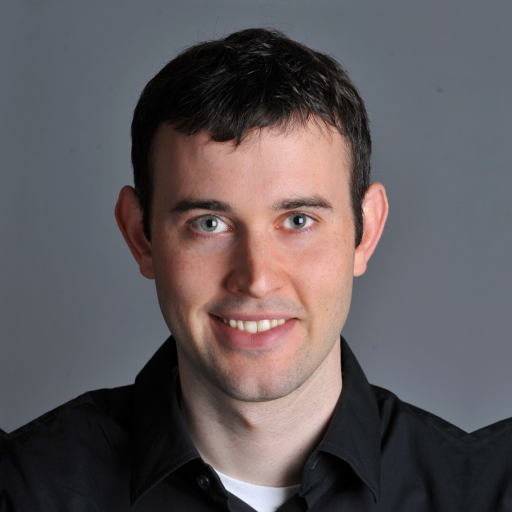
\includegraphics[width=\textwidth]{outputs/part2_4/face-on-apple/second_image.png}
    \caption{Apple.}
  \end{subfigure}\hfill
  \begin{subfigure}[b]{0.22\textwidth}
    
\includegraphics[width=\textwidth]{outputs/part2_4/face-on-apple/mask.png}
    \caption{Irregular mask.}
  \end{subfigure}\hfill
  \begin{subfigure}[b]{0.22\textwidth}
    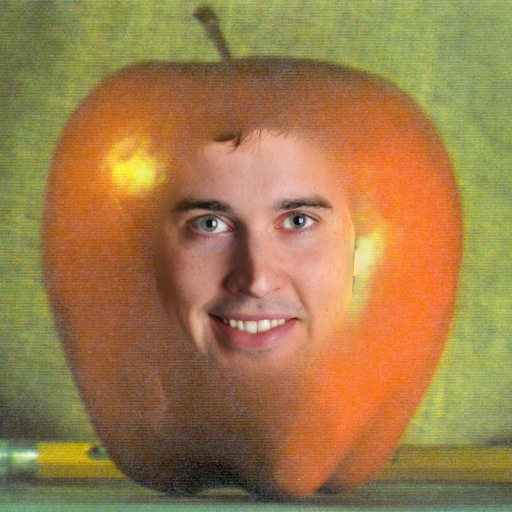
\includegraphics[width=\textwidth]{outputs/part2_4/face-on-apple/blended.png}
    \caption{Blended.}
  \end{subfigure}
  \caption{\textbf{Face-on-Apple blend.}
    An irregular three-ellipse mask places the portrait onto the apple;
    the blended result softens the transition at all frequency scales.}
  \label{fig:face_blend}
\end{figure}

\begin{figure}[H]
  \centering
  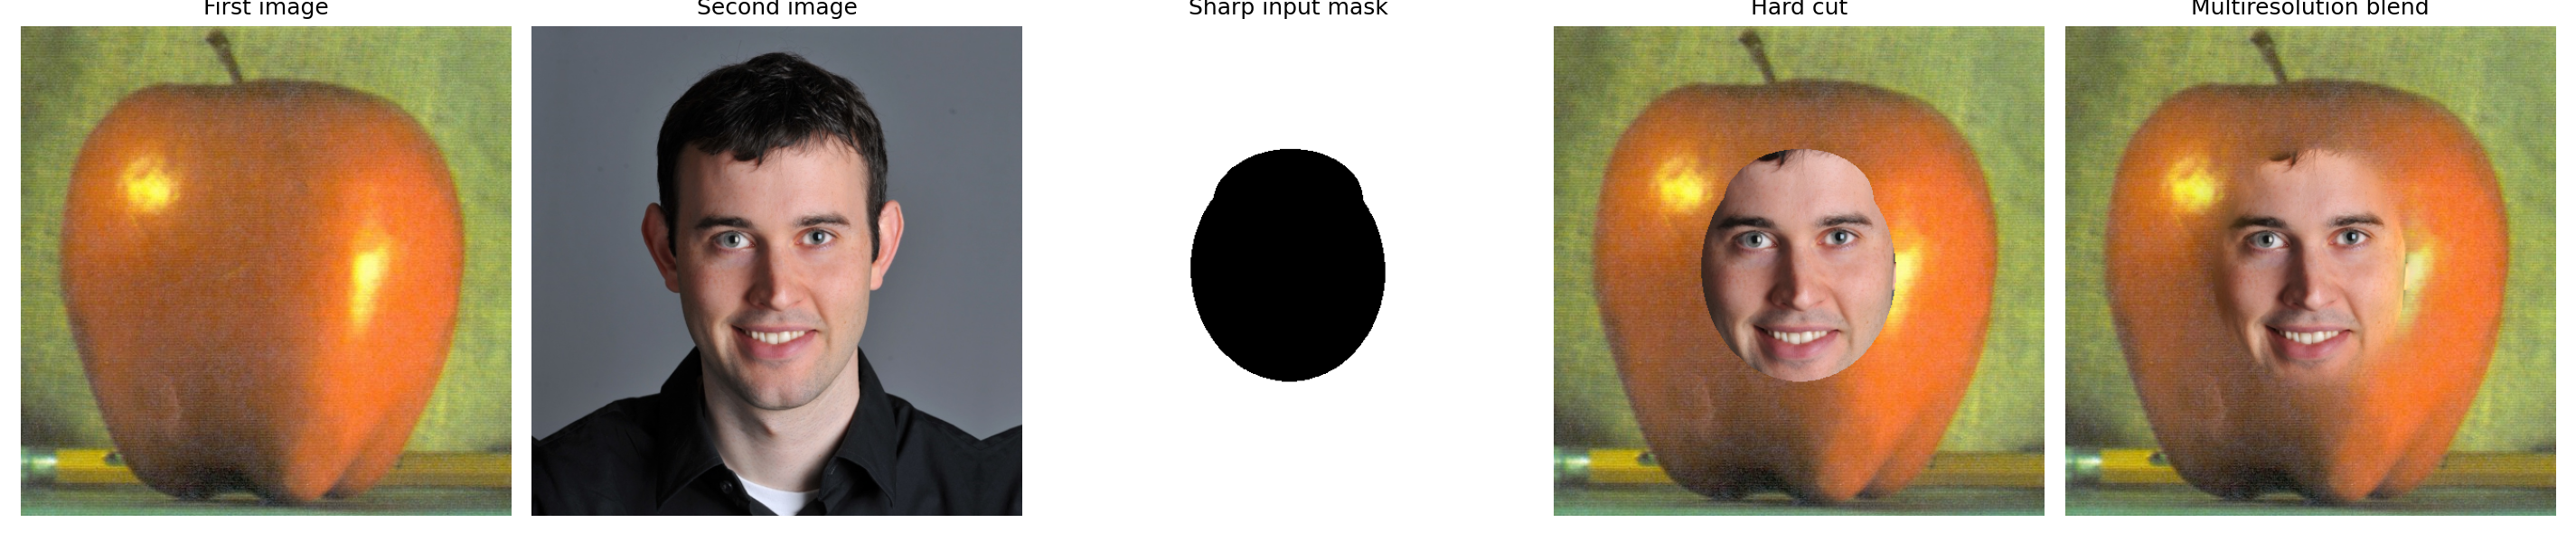
\includegraphics[width=\textwidth]{outputs/part2_4/face-on-apple/comparison.png}
  \caption{Face-on-Apple: hard cut (left) vs.\ multiresolution blend (right).}
  \label{fig:face_cmp}
\end{figure}

\subsubsection{Discussion \texorpdfstring{---}{-} Why Multiresolution Blending Works}

\paragraph{The fundamental problem with a hard cut.}
A sharp boundary has energy at \emph{all} spatial frequencies.  To hide a
seam, the transition width must equal the spatial wavelength of each frequency
band: high frequencies need a \emph{narrow} transition; low frequencies need
a \emph{wide} one.  A single fixed blur width cannot achieve both simultaneously.

\paragraph{The multiresolution solution.}
The Gaussian pyramid naturally widens the mask's transition at each coarser
level:
\[
  \text{transition width at level }k \;\propto\; 2^k \cdot \sigma_{\text{original}}.
\]
Blending the Laplacian pyramid of each source image with this scale-dependent
mask gives every frequency band its own appropriate transition width.  The
reconstructed composite therefore has no visible seam at \emph{any} scale.

\paragraph{Comparison with hard cut.}
All four blends show the same pattern: the hard cut produces a stark colour or
texture discontinuity at the mask boundary, while the multiresolution blend
produces a smooth, natural-looking transition.  The effect is most striking in
the Apple--Orange blend, where the red-vs-orange colour difference would
otherwise produce a vivid step edge.

%%=============================================================
\section{Part 3: Seam Carving}
%%=============================================================

\subsection{Part 3.1 \texorpdfstring{---}{-} Finding and Removing Seams}

A \emph{seam} is a vertically connected path of one pixel per row.  Seam
carving removes the lowest-energy seam repeatedly to reduce image width while
preserving visually important content.  The energy at each pixel is the
gradient magnitude (either finite-difference or DoG).

The optimal seam is found by dynamic programming:
\begin{equation}
  M[i,j] = E[i,j] + \min\bigl(M[i-1,j-1],\; M[i-1,j],\; M[i-1,j+1]\bigr),
  \label{eq:dp}
\end{equation}
where $M[0,j]=E[0,j]$ initialises the top row.  Backtracking from the column
with the minimum value in the last row traces the optimal seam upward.

\textbf{Why exhaustive enumeration is impractical.}
Each row offers up to 3 choices from the pixel selected above, giving
$O(3^H)$ possible seams in an image of height $H$.  For $H=500$ that is
$\sim10^{238}$ paths.  The dynamic program computes the same minimum-cost
path in $O(WH)$ time by reusing sub-problem solutions.

\subsection{Part 3.2 \texorpdfstring{---}{-} Results and Comparisons}

\paragraph{Person outdoors.}
Uniform scaling narrows the person along with the background.  Seam carving
removes more of the surrounding sky and field, leaving the upright figure
close to its original proportions.  Centre cropping also preserves the
figure's shape but discards content at both sides of the frame.

\paragraph{Group photo (failure case).}
Both finite-difference and DoG seams cross the people --- including clothing
and body regions --- rather than removing background only.  The tight framing
leaves few expendable background columns, and gradient magnitude does not
encode the semantic importance of a person.  The carved image therefore
crowds and locally distorts the group.  The DoG energy map is smoother than
the finite-difference map, but smoothing does not prevent seams from crossing
the subjects.

Full comparison images, seam overlays, and the Jaccard overlap between the
two energy seam sets are saved under \texttt{outputs/part3\_2/}.

%%=============================================================
\appendix
\section{Implementation Notes}
%%=============================================================

\subsection{Reflection Padding}

All Part~2 convolutions use \texttt{padding\_mode="reflect"} in
\texttt{convolve\_separable}.  Reflected padding mirrors image content across
the boundary, eliminating the artificial intensity jump produced by zero
padding and its associated border artefacts in edge maps.

\subsection{Separable Convolution via SVD}

\texttt{convolve\_separable} detects rank-1 kernels by checking whether the
ratio of the two largest singular values is below \texttt{rank\_tolerance}
$=10^{-10}$.  All Gaussian and binomial kernels are rank-1 (outer products
of 1D vectors), so the fast $O(\sigma)$-per-pixel separable path is always
taken for Gaussian operations.

\subsection{Binomial vs.\ Gaussian Filter in Pyramids}

The pyramid uses the binomial filter $[1,4,6,4,1]/16$ rather than a general
Gaussian.  Both are low-pass and approximately Gaussian; the binomial filter
is an efficient integer-coefficient approximation used in the original
Burt \& Adelson (1983) construction.

\subsection{Reproducibility}

All output images and raw \texttt{.npy} arrays are saved under
\texttt{outputs/}.  Alignment points are cached in
\texttt{outputs/part2\_1/alignment\_points.json} so results are fully
reproducible without re-running the interactive alignment UI.

%% References -------------------------------------------------
\begin{thebibliography}{9}
\bibitem{BurtAdelson1983}
  P.J.\ Burt and E.H.\ Adelson,
  ``The Laplacian pyramid as a compact image code,''
  \textit{IEEE Transactions on Communications},
  vol.~31, no.~4, pp.~532--540, 1983.
\end{thebibliography}

\end{document}
